%------------------------------------
% Dario Taraborelli
% Typesetting your academic CV in LaTeX
%
% URL: http://nitens.org/taraborelli/cvtex
% DISCLAIMER: This template is provided for free and without any guarantee
% that it will correctly compile on your system if you have a non-standard
% configuration.
% Some rights reserved: http://creativecommons.org/licenses/by-sa/3.0/
%------------------------------------

%!TEX TS-program = xelatex
%!TEX encoding = UTF-8 Unicode

\documentclass[11pt, letterpaper]{article}
\usepackage{fontspec}
\usepackage{wrapfig}
\usepackage{etoolbox}

% CONDITIONAL TO SHOW REFERENCES OR NOT
\newtoggle{showreferences}
%\toggletrue{showreferences}
\togglefalse{showreferences}

% DOCUMENT LAYOUT
\usepackage{geometry}
%\geometry{a4paper, textwidth=5.5in, textheight=8.5in, marginparsep=7pt, marginparwidth=.6in}
\geometry{letterpaper, textwidth=5.9in, textheight=9.0in, marginparsep=7pt, marginparwidth=.7in, includehead}
\setlength\parindent{0in}

% FONTS
\usepackage{xunicode}
\usepackage{xltxtra}
\defaultfontfeatures{Mapping=tex-text} % converts LaTeX specials (``quotes'' --- dashes etc.) to unicode
\setromanfont[Ligatures={Common}, Numbers={OldStyle}]{Hoefler Text}
\setmonofont[Scale=0.8]{Monaco}
\setsansfont[Scale=0.9]{Optima Regular}

% ---- CUSTOM AMPERSAND
\newcommand{\amper}{{\fontspec[Scale=.95]{Hoefler Text}\selectfont\itshape\&}}
% ---- MARGIN YEARS
\usepackage{marginnote}
\newcommand{\years}[1]{\marginnote{\scriptsize #1}}
\renewcommand*{\raggedrightmarginnote}{}
\setlength{\marginparsep}{7pt}
\reversemarginpar

\newenvironment{packed_itemize}{
\begin{itemize}
  \setlength{\itemsep}{1pt}
  \setlength{\parskip}{0pt}
  \setlength{\parsep}{0pt}
}{\end{itemize}}

% HEADINGS
\usepackage{sectsty}
\usepackage[normalem]{ulem}
\sectionfont{\sffamily\mdseries\bfseries\Large\underline}
\subsectionfont{\sffamily\mdseries\bfseries\scshape\large}
\subsubsectionfont{\rmfamily\bfseries\upshape\normalsize}

% PDF SETUP
% ---- FILL IN HERE THE DOC TITLE AND AUTHOR
%\PassOptionsToPackage{hyphens}{url}\usepackage[xetex, bookmarks, colorlinks, breaklinks, pdftitle={Chad A. Steed - vita},pdfauthor={Chad A. Steed}]{hyperref}
\usepackage[usenames, dvipsnames]{xcolor}
% \usepackage[xetex, bookmarks, colorlinks, breaklinks, pdftitle={Chad A. Steed - vita},pdfauthor={Chad A. Steed}]{hyperref}
\usepackage[xetex, bookmarks, breaklinks, pdftitle={Chad A. Steed - vita},pdfauthor={Chad A. Steed}]{hyperref}
%\hypersetup{linkcolor=blue,citecolor=blue,filecolor=black,urlcolor=blue}
% \hypersetup{linkcolor=Maroon,citecolor=Maroon,filecolor=black,urlcolor=Maroon}
\hypersetup{linkcolor=Purple,citecolor=Purple,filecolor=black,urlcolor=Purple}
\renewcommand{\descriptionlabel}[1]{\hspace{\labelsep}\textsc{#1}}

% \usepackage{sparklines}

\usepackage{lastpage}
\usepackage{fancyhdr}
\pagestyle{fancy}

\fancypagestyle{firststyle}
{
    \fancyhf{}
    \rfoot{\small \thepage\ / \pageref{LastPage} • \today}
}

\fancyhf{}
%\lhead{\small Chad A. Steed, Ph.D.}
\rhead{\small Chad A. Steed • Curriculum Vitae}
%\chead{\small Research and Teaching Statements}
%\chead{\small \nouppercase\leftmark}
\rfoot{\small \thepage\ / \pageref{LastPage} • \today}
%\lfoot{\small Chad A.\ Steed}
%\lfoot{\small \today}
%{\scriptsize  Last updated on \today\- •\-
%\lfoot{\small Last Updated: \today}
%\rfoot{\small \href{http://cda.ornl.gov/steed/personal/}{http://cda.ornl.gov/steed/personal/}}
%\renewcommand{\footrulewidth}{0.01cm}
\renewcommand{\headrulewidth}{0cm}
%\renewcommand\footrule{\begin{minipage}{1\textwidth}
%\hrule width \hsize height 2pt \kern 1mm \hrule width \hsize
%\end{minipage}\par}%

% DOCUMENT
\begin{document}
\thispagestyle{firststyle}

\begin{tabbing}
    {\sffamily \LARGE \textbf{CHAD A.\ STEED}} \` {\sffamily \LARGE CURRICULUM VITAE}
\end{tabbing}

\begin{wrapfigure}{r}{0.38\textwidth}
  \vspace{-30pt}
  \begin{center}
    %\includegraphics[width=0.28\textwidth]{chad2.jpg}
    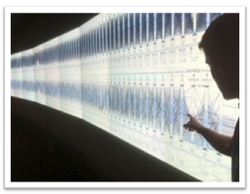
\includegraphics[width=0.4\textwidth]{climate-framed.png}
  \end{center}
  \vspace{-20pt}
\end{wrapfigure}

% VISTA Laboratory\\
Computer Science and Mathematics Division\\
Oak Ridge National Laboratory\\
P.O. Box \texttt{2008}, MS-\texttt{6164}\\
% One Bethel Valley Rd.\\
Oak Ridge, TN \texttt{37831-6164}
U.S.A.\\[.2cm]
Phone: \texttt{865-574-7168}\\
% Cell: \texttt{865-335-1231}\\
% Email: \href{mailto:csteed@acm.org}{csteed@acm.org}\\[.2cm]
Email: \href{mailto:steedca@ornl.gov}{steedca@ornl.gov}\\[.2cm]
\textsc{Website}: \href{https://csteed.com}{https://csteed.com}\\
\textsc{LinkedIn}: \href{https://www.linkedin.com/in/chadsteed}{https://www.linkedin.com/in/chadsteed}\\
\textsc{Twitter}: \href{https://twitter.com/docchad}{https://twitter.com/docchad}\\
\textsc{ORCID}:
\href{http://orcid.org/0000-0002-3501-909X}{http://orcid.org/0000-0002-3501-909X}\\
\textsc{Google Scholar}: \href{http://scholar.google.com/citations?user=DF2gMWkAAAAJ}{http://scholar.google.com/citations?user=DF2gMWkAAAAJ}\\
\textsc{ResearchGate}: \href{https://www.researchgate.net/profile/Chad\_Steed2}{https://www.researchgate.net/profile/Chad\_Steed2}

% \textbf{I am a citizen of the United States.  I hold TS/SCI and Q security clearances.}

\section*{Areas of specialization}
Data Science and Wrangling • Visual Analytics • Interactive Data Visualization • Machine Learning • Statistical Analysis • Cyber Security • Cyber Physical • Database Systems • Climate Science • Text Mining • Computer Graphics • Geographic Systems • Graphic Design

\section*{Technical Skills}
JavaScript • Node.js • D3.js • React.js • jQuery • Electron.js • Jekyll • Pandas • Python • Java • C/C++ • CSS • HTML • Elastic • HDF5 • NetCDF • SQL and NoSQL Databases • OpenGL • Git • Maven • LaTeX • Eclipse • IntelliJ IDEA • Processing • Matlab • R • OmniGraffle • Adobe Creative Suite

\section*{Honors \amper{} Awards}
\noindent\years{2018}MSU Bagley College of Engineering Distinguished Fellow\\
\years{2017}Inducted into the Petal High School Academic Hall of Fame\\
\years{2016}ORNL Best Director's Research \amper{} Development Poster Award\\
\years{2015}R\amper{}D 100 Award Finalist (for CoNNECT energy analytics system)\\
\years{2014}ORNL Early-Career Researcher Award\\
\years{2014}ORNL Technology Commercialization Award\\
\years{2014}ORNL Significant Event Award (SEA) (for successful ACME project demonstration)\\
\years{2014}Elsevier Computers \& Geosciences Journal 2013 Best Paper Award\\
\years{2013}ORNL Technology Commercialization Award\\
\years{2013}R\amper{}D 100 Award (for DTHSTR text recommender algorithm)\\
\years{2013}ORNL Significant Event Award (SEA) (for development and licensing of DTHSTR)\\
\years{2002-2009}NRL Merit Award\\
\years{2008}Inductee, Upsilon Pi Epsilon Honor Society\\
\years{2005-2007}NRL Select Graduate\\
\years{2005}NRL Technology Transfer Award (for GDBV Project)\\
\years{1999}Lockheed Martin Lightning Award (for DBDB-V Project)\\
\years{1999}``Best of Show'' Painting Award in USM Fine Art Dept. Student Art Show\\
\years{1997}USM College of Science and Technology Scholar

\section*{Education}
\noindent\years{2005--2008}\textsc{Ph.D.} in Computer Science (Concentration:
Computer Graphics and Visualization)\\
Mississippi State University, Starkville, MS\\
\emph{Dissertation Title:} ``Development of a Geovisual Analytics Environment using Parallel Coordinates
with Applications to Tropical Cyclone Analysis''\\
\emph{Advisor:} J.\ Edward Swan II\\
\emph{Committee:} T.J.\ Jankun-Kelly, Robert J.\ Moorhead, Edward B.\ Allen, and
Patrick J.\ Fitzpatrick\\

\years{2002--2004}\textsc{M.S.} in Hydrographic Science\\
The University of Southern Mississippi, Hattiesburg, MS\\
\emph{Project Title:} ``A Hydrographic Survey of the Pearl River from Stennis Space Center to the I-10 Bridge''\\

\years{1994--1999}\textsc{B.S.} in Software Engineering (Minor: Fine Art), \emph{Honors}\\
The University of Southern Mississippi, Hattiesburg, MS

\section*{Professional Experience}
\noindent\years{2010--present\\40 hrs/week}Senior Research Staff and Director of the VISTA Data Exploration Laboratory\\
Computer Science and Mathematics Division\\
National Security Sciences Directorate (matrix appointment)\\
Oak Ridge National Laboratory, Oak Ridge, TN\\[.2cm]
I am the Director of the Visual Informatics for Science and Technology Advances (VISTA) Laboratory and a Senior Visual Analytics Researcher in the Computer Science and Mathematics Division at ORNL. I also have a matrix appointment to the National Security Sciences Directorate at ORNL, and I hold two Joint Faculty Appointments to the University of Tennessee, where I periodically mentor students and teach computer science courses. As the founding Director of the VISTA Lab, I am responsible for leading a collaborative data exploration laboratory that serves as a hub for advanced data visualization expertise at ORNL. My research focuses on creating new visual analytics techniques that blend data visualizations, machine learning, and scalable databases to support effective exploratory data analysis. I apply these techniques to multi-disciplinary domains of national significance, namely cyber security, healthcare, materials science, publication mining, climate science, high performance computing, quantum computing, and manufacturing.\\
\underline{Responsibilities}: Building a community of data visualization specialists across multiple directorates at ORNL; Leading VISTA lab operations; Internal data science consulting with ORNL domain experts and leadership; Conducting research and development at both the Principal Investigator and Investigator levels; Active in the full scope of data science research and development; Establishing and maintaining funding sources; sharing technical direction and leadership of the laboratory; publishing, presenting, and demonstrating to academic, industry, and military communities; mentoring students and junior research staff; management of equipment acquisition and maintenance; performing professional service activities; recruiting and hiring new employees; line management of data science professionals; liaison to other divisions at ORNL.\\

\years{2001-2010\\40 hrs/week}Computer Scientist\\
Geospatial Science and Technology Branch\\
Marine Geosciences Division\\
Naval Research Laboratory, Stennis Space Center, MS\\[.2cm]
At NRL, my primary activity was developing visual analytics systems and
interaction techniques for environmental data analysis.  Specifically, I
developed visual analytics solutions for studying tropical cyclone climate
data, oceanographic data, acoustic model sensitivity, and bathymetry data.  I
also developed illustrative visualization techniques for ocean data sets and
new environmental database architectures for bathymetric, hydrographic,
geophysical, ambient noise, seafloor characterization, and unmanned vehicles.\\
\emph{\underline{Responsibilities}}:  Conducted research and development at both the
Principal Investigator and Investigator levels; established and maintained
funding sources; shared technical direction and leadership of the
laboratory; published, presented, and demonstrated to academic, professional,
and military communities; management and supervision of full-time employees
and graduate student interns (usually over the summer); managed equipment
acquisition and maintenance; professional service activities; as a contracting
officer technical representative (COTR), oversaw and provided technical
direction to contractors.\\

\years{1999-2001\\40 hrs/week}Software Engineer\\
Scientific Systems\\
Lockheed Martin, Stennis Space Center, MS\\[.2cm]
After a summer internship, during which I developed an
interactive map application to visualize the World Vector Shoreline Plus
(WVS+) database, I was hired to serve as the Principal Investigator on a new
project to transition the Digital Bathymetric Data Base Variable Resolution
(DBDBV) to the Hierarchical Data Format Version 5 (HDF5) format.  This project
included a comparison of the HDF5 scientific format to other comparable
formats (e.g., GeoTIFF, flat-file), design and development of the new database
model and APIs, and development of database utilities.  This project also
included the development of both a standalone and web-based database
visualization / access application.  I was the Principal Investigator for
the Naval Oceanographic Office's (NAVOCEANO) DBDBV (version 3 and 4) and Mine
Warfare Bottom Sediment Type (BST) database.

\section*{Affiliations and Joint Appointments}

\years{2018--2019}Division Science Council\\
Computer Science and Mathematics Divison\\
Oak Ridge National Laboratory, Oak Ridge, TN\\

\years{2017--present}Joint Faculty Appointment\\
The Bredesen Center for Interdisciplinary Research and Graduate Education\\
The University of Tennessee, Knoxville, TN\\

\years{2017--2018}Division Hiring Committee\\
Computer Science and Mathematics Divison\\
Oak Ridge National Laboratory, Oak Ridge, TN\\

\years{2013--present}Joint Faculty Appointment\\
Electrical Engineering and Computer Science Department\\
The University of Tennessee, Knoxville, TN\\

\years{2013--present}Research Affiliate\\
Climate Change Science Institute\\
Oak Ridge National Laboratory, Oak Ridge, TN\\

\years{2012--present}Adjunct Professor\\
Department of Computer Science and Engineering\\
Mississippi State University, Mississippi State, MS\\

\years{2012--2016}Research Affiliate\\
Center for Intelligent Systems and Machine Learning\\
College of Engineering, The University of Tennessee, Knoxville, TN\\

\years{2009}Adjunct Faculty\\
School of Computing\\
University of Southern Mississippi, Hattiesburg, MS

\section*{Grants \amper{} Contracts}
\begin{sloppypar}
PI or Co-PI on \texttt{39} grants or contracts for a total of \$\texttt{14.1}M
% \begin{sparkline}{4}
% \sparkspike .083 10
% \sparkspike .25 .55
% \sparkspike .417 1
% \sparkspike .583 .62
% \sparkspike .75 .42
% \sparkspike .917 .5
% \end{sparkline}
\\
Lead PI on \texttt{17} grants or contracts totaling \$\texttt{7.1}M\\
\\
\noindent\years{2020}\emph{Principal Investigator}, ``Visual Informatics for Science and Technology (VISTA) Laboratory,'' ORNL,
\$\texttt{250,000}\\
\years{2020}\emph{Investigator}, ``Virtual Anesthesiology,'' DoD,
\$\texttt{75,000} (Lead PI: Tom Potok, ORNL).\\
\years{2019--2020}\emph{Investigator}, ``Nuclear Nonproliferation Data Science,'' NNSA,
\$\texttt{250,000} (Lead PIs: Jeremy Patterson \& Philip Bingham, ORNL).\\
\years{2019--2020}\emph{Investigator}, ``Power Grid Security,'' DOE,
\$\texttt{250,000} (Lead PI: Mason Rice, ORNL).\\
\years{2019}\emph{Investigator}, ``Health Information Technology Advanced Analytics,'' U.S.~Dept.~of Veterans Affairs,
\$\texttt{150,000} (Lead PI: Edmon Begoli, ORNL).\\
\years{2017--2020}\emph{Principal Investigator}, ``SciDAC RAPIDS Task: Temporal and Multivariate Visual Analysis,'' DOE ASCR,
\$\texttt{300,000}.\\
\years{2017--2019}\emph{Principal Investigator}, ``Publication Mining,'' DOE,
\$\texttt{700,000} (Co-PIs: Tom Potok and Robert Patton, ORNL).\\
\years{2017--2018}\emph{Principal Investigator}, ``New Multi-modal Interactive Data Visualization Techniques for Scientific Data Analysis,'' ORNL Seed Project,
\$\texttt{190,000} (Co-PIs: John Goodall, Junghoon Chae, and Steven Hahn, ORNL).\\
\years{2016--2018}\emph{Investigator}, ``Cyber Analytics Techniques and Tools,'' DOE,
\$\texttt{400,000} (Lead PI: John Goodall, ORNL).\\
\years{2016--2017}\emph{Principal Investigator}, ``Visualization Science Advisor to ORNL's Spallation Neutron Source,'' ORNL SNS,
\$\texttt{80,000}.\\
\years{2015--2017}\emph{Investigator}, ``Data Analytics for Additive
Manufacturing,'' ORNL Manufacturing Demonstration Facility,
\$\texttt{400,000} (Lead PI: Ryan DeHoff, ORNL).\\
\years{2015--2016}\emph{Principal Investigator}, ``In Situ Visual Analytics for Transformative
Extreme Scale Science,'' ORNL LDRD,
\$\texttt{645,000} (Co-PIs: Jamison Daniel, Dali Wang, Scott Atchley, Brian
Smith, and Justin Beaver, ORNL).\\
\years{2015--2016}\emph{Investigator}, ``Algorithms for Context-specific Analysis of
Heterogeneous Unstructured Big Health Data,'' ORNL LDRD,
\$\texttt{700,000} (Lead PI: Georgia Tourassi, ORNL).\\
\years{2014--2016}\emph{Principal Investigator}, ``Visual Analytics
of Complex Systems,'' DOD,
\$\texttt{600,000} (Co-PI: Justin Beaver, Joel Reed, ORNL).\\
\years{2013--2014}\emph{Principal Investigator}, ``Interactive Analysis
of High Throughput, Unstructured Information Streams,'' ORNL LDRD,
\$\texttt{900,000} (Co-PIs: John Goodall, Robert Patton, Thomas Potok, and
Christopher Symons, ORNL).\\
\years{2012}\emph{Investigator}, ``A Scalable Framework for Timely
Discovery and Situational Understanding of Cyber Attacks,'' ORNL LDRD,
\$\texttt{350,000} (Lead PI: John Goodall, ORNL).\\
\years{2011--2012}\emph{Investigator}, ``Citizen Engagement for Energy
Efficient Communities (CoNNECT),'' ORNL LDRD, \$\texttt{320,000} (Lead PI: Olufemi A.
Omitaomu, ORNL).\\
\years{2011--2012}\emph{Investigator (Visualization Research Lead)}, ``CMS
Knowledge Discovery Infrastructure,'' Center for Medicare and Medicaid
Services (CMS), \$\texttt{200,000} (\$\texttt{18}M project total) (Lead PI: Wade McNair, ORNL).\\
\years{2011-2012}\emph{Principal Investigator}, ``Multi-State Sharing
Initiative,'' DHS S\amper{}T Southeast Region Research Initiative, \$\texttt{300,000}
(Co-PIs: Christopher Symons and Frank DeNap, ORNL).\\
\years{2011}\emph{Investigator (Visualization Task Lead)}, ``Scalable
Connections for Diverse Information Stores: Knowledge Efficiencies for
Streamlining National Health Informatics,'' ORNL LDRD, \$\texttt{150,000} (Lead PI:
Wade McNair, ORNL).\\
\years{2011--2013}\emph{Investigator}, ``Climate Science for a Sustainable Energy
Future,'' DOE Office of Science, \$\texttt{300,000} (Lead PI:
Peter Thornton, ORNL).\\
\years{2010--2014}\emph{Investigator}, ``Ultra-scale Visualization Climate
Data Analysis Tools,'' DOE Office of Science, \$\texttt{350,000} (Lead PI: Dean Williams,
LLNL).\\
\years{2010--2011}\emph{Principal Investigator}, ``Massively Parallel Algorithms for
Scalable Exascale Data Analysis,'' ORNL LDRD, \$\texttt{720,000} (Lead PI: Cathy Jiao,
ORNL).\\
\years{2010--2011}\emph{Investigator}, ``Multi-State Sharing Initiative,''
DHS S\amper{}T Southeast Region Research Initiative, \$\texttt{150,000} (Lead PI:
Frank DeNap, ORNL).\\
\years{2010}\emph{Investigator}, ``Scale Dependency in Dynamical Downscaling
of Extreme Climate Events over Complex Topography,'' ORNL LDRD, \$\texttt{200,000}
(Lead PI: Tony King, ORNL).\\
\years{2010}\emph{Principal Investigator}, ``Visual Analytics for Undersea
Warfare Planning Study,'' PEO-C4I \amper{} Space PMW-120 Tactical Oceanographic
Capabilities / Undersea Warfare, \$\texttt{40,000}.\\
\years{2010}\emph{Investigator}, ``Bathymetry/Hydrography Uncertainty
Normalization,'' PEO-C4I \amper{} Space PMW-120 METOC Futures Program,
\$\texttt{180,000} (Lead PI: Paul Elmore, ORNL).\\
\years{2006--2010}\emph{Principal Investigator}, ``Geophysical Data Base
Variable Resolution Version 2,'' PEO-C4I \amper{} Space PMW-120 Ocean Bottom
Characterization Initiative, \$\texttt{540,000}.\\
\years{2008--2010}\emph{Principal Investigator}, ``Autonomous Underwater
Vehicle Bathymetry,'' PEO-C4I \amper{} Space PMW-120 LBSF\amper{}I Program,
\$\texttt{755,000} (Co-PIs: Brian Bourgeois, Will Avera, Paul Elmore, NRL).\\
\years{2008--2010}\emph{Principal Investigator}, ``Undersea Semi-Submersible
(USS) Vehicle,'' PEO-C4I \amper{} Space PMW-120 Congressional Plus-up
Project, \$\texttt{200,000} (Co-PIs: Mike Harris and Will Avera, NRL).\\
\years{2006--2009}\emph{Investigator}, ``OAML Bathymetric Data Fusion,''
PEO-C4I \amper{} Space METOC Futures Program, \$\texttt{472,000} (Lead PI: Paul
Elmore, NRL).\\
\years{2008}\emph{Investigator}, ``Transparent Urban Structures II,'' Office
of Naval Research, \$\texttt{560,000} (Lead PI: Kevin Shaw, NRL).\\
\years{2008}\emph{Investigator}, ``Metrics to Evaluate the Effectiveness of
Distributed AUV Sensors,'' NRL Base Program 6.2, \$\texttt{20,000} (Lead PI: Josette
Fabre, NRL).\\
\years{2007}\emph{Investigator}, ``Autonomous Underwater Vehicle Data
Acquisition and Planning,'' PEO-C4I \amper{} Space PMW-180 LBSF\amper{}I,
\$\texttt{100,000} (Lead PI: Michael Harris, NRL).\\
\years{2005--2006}\emph{Principal Investigator}, ``Shipping Noise Data Base
(SNDB),'' PEO-C4I \amper{} Space PMW-180, \$\texttt{211,000}.\\
\years{2004--2005}\emph{Investigator}, ``AQS-20 Through-The-Sensor Rapid
Transition Project,'' PEO-C4I \amper{} Space PMW-150, \$\texttt{1,200,000} (Lead PI:
Michael Harris, NRL).\\
\years{2003--2004}\emph{Principal Investigator}, ``Geophysical Data Base
Variable Resolution,'' SPAWAR PMW-150, \$\texttt{345,000}.\\
\years{2001--2002}\emph{Principal Investigator}, ``Precision Underwater
MApping System (PUMA)--Tactical Environmental Data Server (TEDS) System,''
SPAWAR PMW-150, \$\texttt{340,000}.
\end{sloppypar}

\section*{Open Source Projects}

\years{2020-Present}COVID19Vis,
\href{https://github.com/ORNL/COVID19Vis}{https://github.com/ORNL/COVID19Vis}.\\
Description: Several dynamic visualizations of COVID-19 statistics deployed online at.\\
Web Application: \href{https://ornl.github.io/COVID19Vis/}{https://ornl.github.io/COVID19Vis/}\\
License: MIT License\\
\years{2020-Present}ORAgendaVis,
\href{https://github.com/ORNL/ORAgendaVis}{https://github.com/ORNL/ORAgendaVis}.\\
Description: Timeline visualizations of ORNL Laboratory Initiatives.\\
Web Application: \href{https://ornl.github.io/ORAgendaVis/}{https://ornl.github.io/ORAgendaVis/}\\
License: MIT License\\
\years{2019-2020}VitalVis,
\href{https://github.com/ORNL/VitalVis}{https://github.com/ORNL/VitalVis}.\\
Description: Web-based visual analytics system for exploring patient vitals streams as time series and multivariate visualizations.\\
Web Application: \href{https://ornl.github.io/VitalVis/}{https://ornl.github.io/VitalVis/}\\
License: MIT License\\
\years{2019-2020}Top500Vis,
\href{https://github.com/csteed/Top500Vis}{https://github.com/csteed/Top500Vis}.\\
Description: Web-based visualizations of the Top 500 supercomputing list.\\
Web Application: \href{http://csteed.com/Top500Vis/}{http://csteed.com/Top500Vis/}\\
License: MIT License\\
\years{2016-Present}CrossVis,
\href{http://github.com/ORNL/CrossVis}{http://github.com/ORNL/CrossVis}.\\
Description: Expanded version of the EDEN visual analytics tool for interactive exploratory data analysis.\\
License: MIT License\\
\years{2016-2017}Falcon,
\href{http://github.com/csteed/falcon}{http://github.com/csteed/falcon}.\\
Description: A visual analytics tool for interactive analysis of large time series data.\\
License: MIT License\\
\years{2012-2016}Exploratory Data analysis ENvironment (EDEN),
\href{http://github.com/csteed/eden}{http://github.com/csteed/eden}.\\
Description: A visual analytics tool for interactive analysis of large scale multivariate
data sets.\\
License: UT-Battelle BSD License\\
\years{2015}Storm Brush,
\href{http://github.com/csteed/stormbrush}{http://github.com/csteed/stormbrush}.\\
Description: A collection of algorithms for visualizing tropical cyclone
information using techniques inspired by Impressionists paintings.\\
License: MIT License\\
\years{2014}MultiVar,
\href{http://github.com/csteed/multivar}{http://github.com/csteed/multivar}.\\
Description: A web-based framework to investigate various ways to encode
multivariate climate simulation data using the visual attributes of glyphs.\\
License: MIT License\\

Several other open source projects are available online:
\begin{packed_itemize}
\item \href{https://csteed.com}{https://csteed.com}
\item \href{http://github.com/csteed/}{http://github.com/csteed/}
\item \href{http://gist.github.com/csteed}{http://gist.github.com/csteed}
\item \href{http://bl.ocks.org/csteed}{http://bl.ocks.org/csteed}
\end{packed_itemize}

%\section*{Publications \amper{} talks}
\section*{Publications}
\texttt{93} research publications
% \begin{sparkline}{4}
% \sparkspike .15 .36
% \sparkspike .3 .36
% \sparkspike .45 .45
% \sparkspike .6 .45
% \sparkspike .75 .27
% \sparkspike .9 .09
% \sparkspike 1.05 .64
% \sparkspike 1.2 .82
% \sparkspike 1.35 .27
% \sparkspike 1.5 .36
% \sparkspike 1.65 .91
% \sparkspike 1.8 1.
% \sparkspike 1.95 .18
% \sparkspike 2.1 .09
% \end{sparkline}\\
(\texttt{11} journal articles,
\texttt{25} conference papers, \texttt{9} referred abstracts,
\texttt{20} workshop or position papers, \texttt{2} book
chapters, \texttt{25} technical reports, and \texttt{1} dissertation),
and \texttt{3} patents.
Most of these publications are available on my web site \href{https://csteed.com/}{https://csteed.com/}.

\subsection*{Journal Articles (\texttt{11})}
\begin{sloppypar}
\noindent\years{2020} \textbf{Chad A.\ Steed}, John R.\ Goodall, Junghoon Chae, and Artem A.\ Trofimov. CrossVis: A Visual Analytics System for Exploring Heterogeneous Multivariate Data with Applications to Materials and Climate Sciences. \emph{Graphics \& Visual Computing}, 3:200013, 2020. doi:\href{https://doi.org/10.1016/j.gvc.2020.200013}{10.1016/j.gvc.2020.200013}\\
\years{2019}Artem A.\ Trofimov, Alison A.\ Pawlicki, Nikolay Borodinov, Shovon Mandal, Teresa J.\ Mathews, Mark Hildebrand, Maxim A.\ Ziatdinov, Katherine A.\ Hausladen, Paulina K.\ Urbanowicz, \textbf{Chad A.\ Steed}, Anton V.\ Ievlev, Alex Belianinov, Joshua K.\ Michener, Rama Vasudevan, and Olga S.\ Ovchinnikova. Deep Data Analytics for Genetic Engineering of Diatoms Linking Genotype to Phenotype via Machine Learning. \emph{Nature Partner Journals Computational Materials}, 5:4, 2019. doi:\href{https://doi.org/10.1038/s41524-019-0202-3}
{10.1038/s41524-019-0202-3}\\
\years{2019}John R.\ Goodall, Eric D.\ Ragan, \textbf{Chad A.\ Steed},
Joel W.\ Reed, G.\ David Richardson, Kelly M.T.\ Huffer, Robert A.\ Bridges, and Jason A. Laska. Situ: Identifying and Explaining Suspicious Behavior in Networks. \emph{IEEE Transactions on Visualization and Computer Graphics}, 25(1), 2019. doi:\href{http://dx.doi.org/10.1109/TVCG.2018.2865029}
{10.1109/TVCG.2018.2865029}\\
\years{2017}\textbf{Chad A.\ Steed}, William Halsey, Ryan Dehoff,
Sean L.\ Yoder, Vincent Paquit, and Sarah Powers.  Falcon: Visual Analysis of Large, Irregularly Sampled, and Multivariate Time Series Data in Additive Manufacturing. \emph{Computers \& Graphics}, 63:50--64, 2017. doi:\href{http://dx.doi.org/10.1016/j.cag.2017.02.005}
{10.1016/j.cag.2017.02.005}\\
\years{2015}Arvind Ramanathan, Laura L.\ Pullum, Tanner C.\ Hobson,
Christopher G.\ Stahl, \textbf{Chad A.\ Steed}, Shannon P.\ Quinn,
Chakra S.\ Chennubhotla, and Silvia Valkova.  Discovering Multi-scale
Co-occurrence Patterns of Asthma and Influenza with Oak Ridge Bio-surveillance
Toolkit. \emph{Frontiers in Public Health}, 3(2015): 182, Oct.\ 2015.
doi:\href{http://dx.doi.org/10.3389/fpubh.2015.00182}
{10.3389/fpubh.2015.00182}\\
\years{2015}Alex Belianinov, Rama K.\ Vasudevan, Evgheni Strelcov,
\textbf{Chad Steed}, Sang Mo Yang, Alexander Tselev, Stephen Jesse,
Michael Biegalski, Galen Shipman, Christopher Symons, Albina Borisevich,
Richard Archibald, Sergei Kalinin.  Big Data and Deep Data in Scanning
and Electron Microscopies: Deriving Functionality from Multidimensional Data
Sets. \emph{Advanced Structural and Chemical Imaging}, 1(6):1--25, 2015.
doi:\href{http://dx.doi.org/10.1186/s40679-015-0006-6}
{10.1186/s40679-015-0006-6}\\
\years{2014}Dali Wang, Yang Xu, Peter Thornton, Anthony King,
\textbf{Chad A.\ Steed}, Lianhong Gu, and Joseph Schuchart.
A Functional Unit Testing Platform for the Community Land Model.
\emph{Environmental Modeling and Software}, 55:25--31, 2014.
doi:\href{http://dx.doi.org/10.1016/j.envsoft.2014.01.015}
{10.1016/j.envsoft.2014.01.015}\\
\years{2013}\textbf{Chad A.\ Steed}, Daniel M.\ Ricciuto, Galen Shipman,
Brian Smith, Peter E.\ Thornton, Dali Wang, and Dean N.\ Williams.
Big Data Visual Analytics for Exploratory Earth System Simulation Analysis.
\emph{Computers \amper{} Geosciences}, 61:71--82, 2013.
doi:\href{http://dx.doi.org/10.1016/j.cageo.2013.07.025}
{10.1016/j.cageo.2013.07.025}
\textbf{\emph{CAGEO 2013 Best Paper Award}}\\
\years{2013}Dean N.\ Williams, Timo Bremer, Charles Doutriaux, John Patchett,
Sean Williams, Galen Shipman, Ross Miller, David R.\ Pugmire, Brian Smith,
\textbf{Chad A.\ Steed}, E.\ Wes Bethel, Hank Childs, Harinarayan Krishnan,
Prabhat, Claudio T.\ Silva, Emanuele Santos, David Koop, Tommy Ellqvist,
Jorge Poco, Berk Geveci, Aashish Chaudhary, Andy Bauer, Alexander Pletzer,
Dave Kindig, Gerald L.\ Potter, and Thomas P.\ Maxwell. The Ultra-scale
Visualization Climate data Analysis Tools (UV-CDAT): Data Analysis and
Visualization for Geoscience Data. \emph{IEEE Computer}. 46(9):68--76, 2013.
doi:\href{http://dx.doi.org/10.1109/MC.2013.119}{10.1109/MC.2013.119}\\
\years{2009}\textbf{Chad A.\ Steed}, Patrick J.\ Fitzpatrick, T.J.\ Jankun-Kelly,
Amber N.\ Yancey, and J.\ Edward Swan II. An Interactive
Parallel Coordinates Technique Applied to a Tropical Cyclone Climate
Analysis. \emph{Computers \amper{} Geosciences}, 35(7):1529--1539, 2009.
doi:\href{http://dx.doi.org/10.1016/j.cageo.2008.11.004}
{10.1016/j.cageo.2008.11.004}\\
\years{2009}\textbf{Chad A.\ Steed}, Patrick J.\ Fitzpatrick, J.\ Edward Swan
II, and T.J.\ Jankun-Kelly. Tropical Cyclone Trend Analysis using Enhanced
Parallel Coordinates and Statistical Analytics. \emph{Cartography and
Geographic Information Science}, 36(3):251--265, 2009.
doi:\href{http://dx.doi.org/10.1559/152304009788988314}{10.1559/152304009788988314}
\end{sloppypar}

\subsection*{Conference Papers (\texttt{25})}
\begin{sloppypar}
\noindent\years{2019}Junghoon Chae, Debsindhu Bhowmik, Heng Ma, Arvind Ramanathan, and \textbf{Chad A.~Steed}. Visual Analytics for Deep Embeddings of Large Scale Molecular Dynamics Simulations. In
\emph{IEEE International Conference on Big Data}, pp.\ pp. 1759-1764, 2019. doi:\href{https://doi.org/10.1109/BigData47090.2019.9006048}{10.1109/BigData47090.2019.9006048}\\
\years{2019}Junghoon Chae, \textbf{Chad A. Steed}, John Goodall, and Steven Hahn. Dynamic Color Mapping with a Multi-scale Histogram: A Design Study with Physical Scientists. In
\emph{Proceedings of the Visualization and Data Analysis Conference}, pp.\ 680-1--680-13, Jan.\ 2019. doi:\href{https://doi.org/10.2352/ISSN.2470-1173.2019.1.VDA-680}{10.2352/ISSN.2470-1173.2019.1.VDA-680}\\
\years{2016}Dali Wang, Zhuo Yao, Yulu Xu, \textbf{Chad A.\ Steed},
Scott Atchley, Jamison Daniel, Brian Smith. In Situ Data Infrastructure for
Scientific Unit Testing Platform.
In \emph{Proceedings of the International Conference on Computational Science},
pp.\ 587--598, June 2016. doi:\href{http://dx.doi.org/10.1016/j.procs.2016.05.344}{10.1016/j.procs.2016.05.344}\\
\years{2016}Arvind Ramanathan, Shannon Quinn, Laura Pullum, and
\textbf{Chad A.\ Steed}. Tracking Alcohol and Marijuana Usage and Behaviors
from Social Media using Oak Ridge Bio-Surveillance Toolkit.
In \emph{Proceedings of the IEEE International Conference on Biomedical and
Health Informatics}, Feb.\ 2016.\\
\years{2015}\textbf{Chad A.\ Steed}, Margaret Drouhard, Justin
Beaver, Joshua Pyle, and Paul L.\ Bogen II. Matisse: A Visual Analytics
System for Exploring Emotion Trends in Social Media Text Streams.
In \emph{Proceedings of the IEEE International Conference on Big Data (IEEE
Big Data 2015)}, pp.\ 807--814, Oct.\ 2015. doi:\href{http://dx.doi.org/10.1109/BigData.2015.7363826}{10.1109/BigData.2015.7363826} (62/368 [18\%] acceptance rate)\\
\years{2014}\textbf{Chad A.\ Steed}, Katherine J.\ Evans, John F.\ Harney,
Brian C.\ Jewell, Galen Shipman, Brian E.\ Smith, Peter E.\ Thornton, and
Dean N.\ Williams. Web-based Visual Analytics for Extreme Scale Climate Science.
In \emph{Proceedings of the IEEE International Conference on Big Data (IEEE Big Data 2014)},
pp.\ 383--392, Oct.\ 2014.
doi:\href{http://dx.doi.org/10.1109/BigData.2014.7004255}{110.1109/BigData.2014.7004255} (49/264 [18\%] acceptance rate)\\
\years{2013}Robert Patton, \textbf{Chad A.\ Steed}, Chris G.\ Stahl, and
Jim N.\ Treadwell. Observing Community Resiliency in Social Media. \emph{The 13th
International Conference on Computational Science and Applications (ICCSA 2013)},
pp.\ 491--501, June 2013.
doi:\href{http://dx.doi.org/10.1007/978-3-642-39640-3\_36}{10.1007/978-3-642-39640-3\_36} \\
\years{2013}Brian Smith, Daniel M.\ Ricciuto, Peter E.\ Thornton, Galen Shipman,
\textbf{Chad Steed}, and Dean Williams. ParCAT: Parallel Climate Analysis Toolkit.
In \emph{Proceedings of the International Conference on Computational
Science}, pp.\ 2367--2375, June 2013.
doi:\href{http://dx.doi.org/10.1016/j.procs.2013.05.408}{10.1016/j.procs.2013.05.408} \\
\years{2012}Arvind Ramanathan, \textbf{Chad A.\ Steed}, Laura L.\ Pullum.
Verification of Compartmental Epidemiological Models using Metamorphic Testing,
Model Checking and Visual Analytics. In \emph{Proceedings of the ASE/IEEE International
Conference on BioMedical Computing (BioMedCom)}, Washington, D.C., Dec.\ 2012.
doi:\href{http://dx.doi.org/10.1109/BioMedCom.2012.18}{10.1109/BioMedCom.2012.18} \\
\years{2012}Songhua Xu, Brian Jewell, \textbf{Chad Steed},
and Jack Schryver. A New Collaborative Tool for Visually Understanding
National Health Indicators. In \emph{Proceedings of the International
Conference on Applied Human Factors and Ergonomics (AHFE)}, San Francisco, CA,
July 2012.\\
\years{2012}\textbf{Chad A. Steed}, Galen Shipman, Peter Thornton, Daniel Ricciuto,
David Erickson, and Marcia Branstetter.  Practical Application of Parallel Coordinates for
Climate Model Analysis. In \emph{Proceedings of the International Conference on Computational
Science}, pp.\ 877--886, June 2012.
doi:\href{http://dx.doi.org/10.1016/j.procs.2012.04.094}
{10.1016/j.procs.2012.04.094} \\
\years{2012}\textbf{Chad A. Steed}, Christopher Symons, Frank DeNap, and
Thomas E. Potok. Guided Text Analysis Using Adaptive Visual Analytics. In
\emph{Proceedings of the Visualization and Data Analysis Conference}, SPIE.
doi:\href{http://dx.doi.org/10.1117/12.904904}{10.1117/12.904904} (24/50 [48\%] acceptance rate)\\
\years{2011}Robert M. Patton, Justin M. Beaver, \textbf{Chad A. Steed},
Thomas E. Potok, and Jim N. Treadwell. Hierarchical Clustering and
Visualization of Aggregate Cyber Data. In \emph{Proceedings of the International
Wireless Communications and Mobile Computing Conference}, pp.\ 1287--1291,
IEEE Computer Society. doi:\href{http://dx.doi.org/10.1109/IWCMC.2011.5982725}
{10.1109/IWCMC.2011.5982725} (35\% acceptance rate)\\
\years{2011}Justin M. Beaver, \textbf{Chad A. Steed}, Robert M. Patton,
Xiaohui Cui, and Matthew Schultz. Visualization Techniques for Computer
Network Defense. In \emph{Proceedings of the Defense \amper{} Security
Symposium}, vol.\ 8019, pp.\ 1--9, SPIE.
doi:\href{http://dx.doi.org/10.1117/12.883487} {10.1117/12.883487}\\
\years{2009}\textbf{Chad A.~Steed}, J. Edward Swan II, T.J. Jankun-Kelly,
and Patrick J. Fitzpatrick. Guided Analysis of Hurricane Trends using
Statistical Processes Integrated with Interactive Parallel Coordinates.  In
\emph{Proceedings of Symposium on Visual Analytics Science and Technology}
(J. Stasko and Jarke J. van Wijk, eds.), Atlantic City, NJ, pp.\ 19--26, IEEE
Computer Society, Oct.\ 2009 (26/ 69 [38\%] acceptance rate; Proceedings
cover page featured a figure from this paper).
doi:\href{http://dx.doi.org/10.1109/VAST.2009.5332586}
{10.1109/VAST.2009.5332586}\\
\years{2009}Art Kleiner, David Alleman, Pete Alleman, and
\textbf{Chad A. Steed}.  Development of a New Unmanned Semi Submersible (USS)
Vehicle. In \emph{Proceedings of Oceans 2009}, pp.\ 1--6, MTS/IEEE.\\
\years{2009}\textbf{Chad A. Steed}, T.J. Jankun-Kelly,  and J. Edward Swan
II. Illustrative Visualization of Hurricane Advisory Information. In
\emph{Proceedings of Oceans 2009}, Biloxi, MS, pp.\ 1-–9, MTS/IEEE, Oct.\ 2009.\\
\years{2005}Costin Barbu, William E. Avera, Dale Bibee, Michael M. Harris,
and \textbf{Chad Steed}. AQS-20 Sonar Processing Enhancement for Bathymetry
Estimation.  In \emph{Proceedings of Oceans 2005}, Washington, D.C., vol.\ 3,
pp.\ 2025-–2029, MTS/IEEE, Sep.\ 2005.
doi:\href{http://dx.doi.org/10.1109/OCEANS.2005.1640057}
{10.1109/OCEANS.2005.1640057}\\
\years{2005}Michael Harris, William Avera, \textbf{Chad Steed}, John Sample,
L. Dale Bibee, Dave Morgerson, Jim Hammack, and Mark Null.  AQS-20
Through-The-Sensor (TTS) Performance Assessment.  In \emph{Proceedings of
Oceans 2005}, Washington, D.C., vol.\ 1, pp.\ 460-–465, MTS/IEEE, Sep.\ 2005.
doi:\href{http://dx.doi.org/10.1109/OCEANS.2005.1639807}
{10.1109/OCEANS.2005.1639807}\\
\years{2005}\textbf{Chad A. Steed}, John Sample, Michael Harris, William
Avera, and L. Dale Bibee. AQS-20 Through-The-Sensor Environmental Data
Sharing.  In \emph{Proceedings of the Defense \amper{} Security Symposium},
Orlando, FL, vol.\ 5778, pp.\ 32-–41, SPIE, Mar.\ 2005.
doi:\href{http://dx.doi.org/10.1117/12.606327}{10.1117/12.606327}\\
\years{2004}Michael Harris, Will Avera, L. Dale Bibee, \textbf{Chad Steed},
John Sample, Mark Null, and Jim Hammack.  Environmental Data Collection,
Sensor to Decision Aid.  In \emph{Sixth International Symposium on Technology
and the Mine Problem}, Monterey, CA, pp.\ 818–-823, Naval Postgraduate
School, May 2004.\\
\years{2004}Stephanie Myrick and \textbf{Chad Steed}.  3D Enhancements for
Visualizing Lane Navigation Performance.  In \emph{Proceedings of the Human
Performance, Situation Awareness, and Automation Technology Conference},
Daytona Beach, FL, pp.\ 248–-252, Lawrence Erlbaum Association, Mar.\ 2004.\\
\years{2003}\textbf{Chad A. Steed}, Chiu-Fu ``Tiger'' Cheng, and David W.
Harvey.  Development of a Flexible, Geophysical Database using HDF5.  In
\emph{Proceedings of Oceans 2009}, Biloxi, MS, pp.\ 1-–6, MTS/IEEE, Oct.\ 2003.\\
\years{2003}\textbf{Chad A. Steed}, Kim Koehler, Dave Harvey, and Bruce
Northridge.  Geophysical Data Base Variable Resolution (GDBV): An
Object-Oriented Database for Dynamic Geo-acoustic Data Storage.  In
\emph{Proceedings of Oceans 2003}, San Diego, CA, pp.\ 132-–140, MTS/IEEE,
Sep.\ 2003. doi:\href{http://dx.doi.org/10.1109/OCEANS.2003.178534}
{10.1109/OCEANS.2003.178534}\\
\years{2002}\textbf{Chad A. Steed}, Kim Koehler, and James E. Braud.
VGRID: A Generic, Dynamic HDF5 Storage Model for Georeferenced Grid Data.
In \emph{Proceedings of Oceans 2002}, Biloxi, MS, pp.\ 900-–907,
MTS/IEEE, Oct.\ 2002. doi:\href{http://dx.doi.org/10.1109/OCEANS.2002.1192087}
{10.1109/OCEANS.2002.1192087}
\end{sloppypar}

\subsection*{Referred Abstracts (\texttt{9})}
\noindent\years{2017}\textbf{Chad A. Steed}, Junghoon Chae, John Goodall, and Steven Hahn.  Improving Scientific Data Analysis Through Multi-touch Enabled Interactive Data Visualization with Applications to Neutron Science.  In \emph{Proceedings of the Workshop on Immersive Analytics at IEEE VIS 2017}, Phoenix, AZ, pp.\ 1--2, Oct.\ 2017.\\
\years{2016}\textbf{Chad A. Steed}, Ryan Dehoff, William Halsey, Sean Yoder, Vincent Paquit, and Sarah Powers.  Advancing Additive Manufacturing Through Visual Data Science.  In \emph{Proceedings of the Symposium on Visualization in Data Science at IEEE VIS 2016}, Baltimore, MD, pp.\ 1--2, Oct.\ 2016.\\
\years{2016}William Halsey, \textbf{Chad A. Steed}, Ryan Dehoff,
Vincent Paquit, and Sean Yoder. Segmented Time Series Visualization Tool for
Additive Manufacturing.  In \emph{IEEE Large Data Analysis and Visualization
(LDAV)Symposium Posters Compendium}, Baltimore, MD, pp.\ 1--2, Oct. 2016.\\
\years{2012}Blake Haugen, Brian Smith, \textbf{Chad A. Steed},
Daniel Ricciuto, Peter E. Thornton, and Galen Shipman.  ParCAT: A Parallel
Climate Analysis Toolkit. \emph{AGU 2012 Fall Meeting}, San Francisco, CA, Dec. 2012.\\
\years{2012}Christopher Maness, \textbf{Chad A. Steed}, and
Olufemi Omitaomu. Practical Web Based Visualization for Comparative Energy
Usage Analysis.  In \emph{IEEE Visualization Conference Compendium}, Seattle, WA,
pp.\ 1--2, IEEE Computer Society.\\
\years{2011}David J. Erickson, Auroop R. Ganguly, Robert
James Oglesby, Evan A. Kodra, Debasish Das, Anthony W. King, Cindy Hays,
\textbf{Chad Steed}, Robert Patton, and Chris Lenhardt. Scale Dependency in
Dynamic Downscaling of Extreme Climate Events over Complex Topography.
Abstract GC24B-05, \emph{AGU 2011 Fall Meeting}, San Francisco, CA,
Dec.\ 2011.\\
\years{2010}Debasish Das, Evan Kodra, Karsten Steinhaeuser, Shih-Chieh Kao,
Auroop R. Ganguly, Marcia L. Branstetter, David J. Erickson, Raymond Flanery,
Maria Martinez Gonzalez, Cynthia Hays, Anthony W. King, Christopher Lenhardt,
Robert Oglesby, Robert M. Patton, Clinton M. Rowe, Alexander Sorokine,
\textbf{Chad Steed}.  Scale Dependency in Dynamic Downscaling of Extreme
Climate Events Over Complex Topography. \emph{AGU Fall Meeting Poster Session},
San Francisco, CA, Dec.\ 2010.\\
\years{2009}\textbf{Chad A. Steed}, T.J. Jankun-Kelly, J. Edward Swan II, and
Robert J. Moorhead. Illustrative Visualization of Hurricane Advisory
Information. In \emph{IEEE Visualization Conference Compendium}, Atlantic City, NJ,
pp.\ 1-–2, IEEE Computer Society, Oct.\ 2009.\\
\years{2007}\textbf{Chad A. Steed}, Patrick J. Fitzpatrick, T.J. Jankun-Kelly,
Amber N. Yancey, and J. Edward Swan II.  Practical Application of Parallel
Coordinates to Hurricane Trend Analysis.  In \emph{IEEE Information Visualization
Conference Compendium}, pp.\ 4–-5, IEEE Computer Society, Oct.\ 2007.

\subsection*{Workshop or Position Papers (\texttt{20})}

\begin{sloppypar}
\noindent\years{2017}Junghoon Chae, Shang Gao, Arvind Ramanathan, \textbf{Chad A.\ Steed}, and Georgia D.\ Tourassi. Visualization for Classification in Deep Neural Networks. In \emph{Proceedings of the Workshop on Visual Analytics for Deep Learning at IEEE VIS 2017}, Pheonix, AZ , Oct.\ 2017.\\
\years{2016}Sarah Powers, Ryan Dehoff, Vincent Paquit,
\textbf{Chad A.\ Steed}, and Derek Kistler. Application of Data Analytics
to Additive Manufacturing.
In \emph{Proceedings of the 11th INFORMS Workshop on Data Mining and
Decision Analytics}, Nashville, TN, Nov.\ 2016.\\
\years{2016}\textbf{Chad A.\ Steed}, Jamison Daniel, Margaret
Drouhard, Thomas Proffen, and Steven Hahn. Immersive Visual Analytics for
Transformative Neutron Scattering Science.
In \emph{Proceedings of the 1st Workshop on Immersive Analytics at IEEE Virtual
Reality 2016}, Greenville, SC, Mar.\ 2016. doi:\href{https://doi.org/10.1109/IMMERSIVE.2016.7932381}
{10.1109/IMMERSIVE.2016.7932381}\\
\years{2016}Shannon Quinn, Arvind Ramanathan, Laura Pullum, and
\textbf{Chad A.\ Steed}. Dr.\ Twitter: The Logistics of Practical Disease
Surveillance using Social Media.
In \emph{Proceedings of the Web-based Public Health Informatics Workshop at
IEEE BHI 2016}, Feb.\ 2016.\\
\years{2015}Blake Haugen, Stephen Richmond, Jakub Kurzak,
\textbf{Chad A.\ Steed}, and Jack Dongarra. Visualizing Execution Traces
with Task Dependencies.
In \emph{Proceedings of the 2nd Workshop on Visual Performance Analysis at SC 15}, Austin, TX, Nov.\ 2015.
doi:\href{http://dx.doi.org/10.1145/2835238.2835240}
{10.1145/2835238.2835240}\\
\years{2015}Margaret Drouhard, \textbf{Chad A.\ Steed}, Steven Hahn,
Thomas Proffen, Jamison Daniel, and Michael Matheson. Immersive Visualization
for Materials Science Data Analysis using the Oculus Rift.
In \emph{Proceedings of the 2nd Workshop on Advances in Software and Hardware for Big Data to Knowledge Discovery at IEEE Big Data 2015}, Santa Clara, CA, pp.\ 2453--2461, Oct.\ 2015. doi:\href{http://dx.doi.org/10.1109/BigData.2015.7364040}{10.1109/BigData.2015.7364040}\\
\years{2015}\textbf{Chad A. Steed}, Justin Beaver, Paul L.\ Bogen II,
Margaret Drouhard, and Joshua Pyle.  Text Stream Trend Analysis using
Multiscale Visual Analytics with Applications to Social Media Systems.
In \emph{Proceedings of the ACM IUI Visual Text Analytics Workshop}, Atlanta,
GA, Mar.\ 2015.\\
\years{2013}\textbf{Chad A.\ Steed}, Thomas E.\ Potok, Laura L.\ Pullum,
Arvind Ramanathan, Galen Shipman, and Peter E. Thornton. Extreme Scale Visual Analytics.
In \emph{Proceedings of the 4th SuperComputing Workshop on Petascale Data Analytics (SC13)},
Denver, CO, Nov.\ 2013.\\
\years{2013}Arvind Ramanathan, Laura L.\ Pullum, \textbf{Chad A. Steed},
Shannon S.\ Quinn, and Chakra S.\ Chennubhotla. Oak Ridge Bio-surveillance Toolkit.
In \emph{Proceedings of IEEE VAST Workshop on Public Health's Wicked Problems:
Can InfoVis Save Lives?}, Atlanta, GA, Oct.\ 2013.\\
\years{2013}Arvind Ramanathan, Laura L.\ Pullum, \textbf{Chad A. Steed},
Shannon S.\ Quinn, Chakra S.\ Chennubhotla, and Tara Parker.
Integrating Heterogeneous Healthcare Datasets and Visual Analytics for Disease
Bio-surveillance and Dynamics. In \emph{Proceedings of the 3rd Interactive
Visual Text Analytics Workshop}, Atlanta, GA, Oct.\ 2013.\\
\years{2013}Dali Wang, Yang Xu, Peter Thornton, Anthony King,
and \textbf{Chad A. Steed}. A Pilot Study on Functional Unit Testing for
Community Land Model. \emph{Computational Data Analytics Workshop (CDAW-13)},
Oak Ridge, TN, Oct.\ 2013.\\
\years{2013}Robert Patton, \textbf{Chad A. Steed}, Chris Stahl.
Visualizing Community Resilience Metrics from Twitter Data. \emph{The 2nd Workshop
on Social Media Visualization (ICWSM-13)}, Boston, MA, Jul.\ 2013.\\
\years{2012}\textbf{Chad A.\ Steed}, Thomas E.\ Potok, Robert M.\ Patton,
John R.\ Goodall, Christopher Maness, James Senter.  Interactive Visual Analysis
of High Throughput Text Streams. In \emph{Proceedings of the 2nd Interactive
Visual Text Analytics Workshop}, Seattle, WA, Oct.\ 2012.
\href{http://research.microsoft.com/en-us/um/people/shliu/tasmc/}
{http://research.microsoft.com/en-us/um/people/shliu/tasmc/}\\
\years{2012}Olufemi A.\ Omitaomu, Christopher S.\ Maness, Ian S.\ Kramer,
Jeffrey B.\ Kodysh, Budhendra L.\ Bhaduri, \textbf{Chad A. Steed},
Rajasekar Karthik, Philip J.\ Nugent, Aaron T.\ Myers. An Integrated Geovisual
Analytics Framework for Analysis of Energy Consumption Data and Renewable
Energy Potentials. In \emph{Proceedings of the GeoSpatial Visual Analytics Workshop at
GIScience}, Columbus, OH, Sep.\ 2012.
\href{http://geoanalytics.net/GeoVA(t)2012/}{http://geoanalytics.net/GeoVA(t)2012/}\\
\years{2009}\textbf{Chad A. Steed}, Patrick J. Fitzpatrick, T.J.
Jankun-Kelly, and J. Edward Swan II. North Atlantic Hurricane Trend Analysis
using Parallel Coordinates and Statistical Techniques.  In \emph{Proceedings of
the GeoSpatial Visual Analytics Workshop}, Park City, UT, pp.\ 1–-4, Sep.\ 2008.
\href{http://geoanalytics.net/GeoVisualAnalytics08/}
{http://geoanalytics.net/GeoVisualAnalytics08/}\\
\years{2008}Paul Elmore and \textbf{Chad A. Steed}.  Algorithm for Bathymetry
Fusion with Uncertainty Assessment.  In \emph{Proceedings of the NRL Technical
Metrics Workshop}, Stennis Space Center, MS, May 2008.\\
\years{2008}\textbf{Chad A. Steed}.  Advanced Visualization Techniques for
Undersea Warfare. In \emph{Proceedings of the NRL Technical Metrics Workshop},
Stennis Space Center, MS, May 2008. \\
\years{2004}Stephanie Myrick and \textbf{Chad Steed}. 3 Dimensional Scene
Reconstruction and Animation using VRML/X3D.  In \emph{Proceedings of
Mississippi Academy of Sciences Annual Meeting}, Biloxi, MS, Mississippi
Academy of Sciences, Feb.\ 2004.\\
\years{2003}Kim Koehler, Michael Harris, Dale Bibee, \textbf{Chad Steed},
and Dave Bates.  Ocean Through The Sensor (TTS) Update.  \emph{SPAWAR PMW-150
Quarterly Newsletter}, pp.\ 1–-11, Space and Naval Warfare Command, Dec.\ 2003.\\
\years{2002}\textbf{Chad A. Steed} and Hillary Mesick. A Method for Overcoming
Discontinuity Between Neighboring UTM Zone Grids.  In \emph{Proceedings of
Mississippi Academy of Sciences Annual Meeting}, Biloxi, MS, Mississippi
Academy of Sciences, Feb.\ 2002.
\end{sloppypar}

\subsection*{Book Chapters (\texttt{2})}
\noindent\years{2016}\textbf{Chad A. Steed}. Interactive Data Visualization.
In \emph{Data Analytics for Intelligent Transportation}. Eds. Mashrur
Chowdhury, Amy Apon, and Kakan Dey. pp. 165--190, 2017.\\
\years{2013}\textbf{Chad A. Steed}, J. Edward Swan II,
Patrick J. Fitzpatrick, and T.J. Jankun-Kelly.  A Visual Analytics Approach
for Correlation, Classification, and Regression Analysis. In \emph{Innovative Approaches
of Data Visualization and Visual Analytics}. Eds. Maolin Huang and Weidong Huang. pp.\ 25--45, 2013.
doi:\href{http://dx.doi.org/10.4018/978-1-4666-4309-3.ch002}{10.4018/978-1-4666-4309-3.ch002}

\subsection*{Technical Reports (\texttt{25})}
\begin{sloppypar}
\noindent\years{2016}\textbf{Chad A.\ Steed}, Ryan Dehoff, William Halsey, Sean Yoder,
Vincent Paquit, and Sarah Powers. Falcon: A Temporal Visual Analytics System Applied to the Analysis of 3D Printer Log Data.  ORNL Technical Report ORNL/TM-2016/393,
Oak Ridge National Laboratory, Oak Ridge, TN, Aug. 2016. 25 pp.\\
\years{2013}Dean N.\ Williams, Andrew Bauer, Aashish Chaudhary, Berk Geveci,
Harinarayan Krishnan, David Bader, Timo Bremer, Charles Doutriaux, Daniel Fedor-Thurman,
Matthew Harris, Elo Leung, Renata McCoy, James Ahrens, Curt Canada, Phil Jones,
Boonthanome Nouanesengsy, John Patchett, Sean Williams, Thomas Maxwell, Gerald Potter,
Cecelia DeLuca, Ryan O'Kuinghttons, Robert Oehmke, David Pugmire, Galen Shipman, Brian Smith,
\textbf{Chad Steed}, Ben Burnett, Aritra Dasgupta, Tommy Ellqvist, David Koop,
Emanuele Marques, Jorge Poco, Remi Rampin, Claudio Silva, Huy Vo, David Kindig, Alexander Pletzer,
Cameron Christensen, Sidharth Kumar, Valerio Pascucci, Giorgio Scorzelli, Brian Summa.
Ultrascale Visualization Climate Data Analysis Tools. LLNL Technical Report
LLNL-TR-643624, Lawrence Livermore National Laboratory, Livermore, CA, Sep. 2013. 96 pp.\\
\years{2012}\textbf{Chad A.\ Steed}, Christopher T.\ Symons,
James K.\ Senter, and Frank A.\ DeNap. Guided Text Search Using Adaptive
Visual Analytics. ORNL Technical Report
\href{http://info.ornl.gov/sites/publications/Files/Pub39480.pdf}{ORNL/TM-2012/479},
Oak Ridge National Laboratory, Oak Ridge, TN, 31 Oct. 2012. 20 pp.\\
\years{2012}\textbf{Chad A.\ Steed}, J.\ Edward Swan II,
Patrick J.\ Fitzpatrick, and T.J.\ Jankun-Kelly.  A Visual Analytics Approach
for Correlation, Classification, and Regression Analysis. ORNL Technical
Report \href{http://info.ornl.gov/sites/publications/Files/Pub24402.pdf}{ORNL/TM-2012/68},
Oak Ridge National Laboratory, Oak Ridge, TN,
21 Feb. 2012. 30 pp.\\
\years{2011}Yu Jiao, Erik Ferragut, Sudharshan Vazhkudai,
Stuart Campbell, Mark Hagen, Stephen Miller, Christopher Griffin, and
\textbf{Chad A. Steed}. Massively Parallel Algorithms for Scalable Exascale
Analysis. ORNL LDRD Report 31964, Oct. 2011. 2 pp.\\
\years{2010}\textbf{Chad A. Steed}, Jeffrey Russell, and J. Paquin
Fabre. Under Sea Warfare Visual Analytics: Fiscal Year 2010 Prototype System
Report. Memorandum Report NRL/MR/7440--10-9285, U.S. Naval Research
Laboratory, Stennis Space Center, MS, 30 Nov. 2010. 13 pp.\\
\years{2010}\textbf{Chad A. Steed}, Chiu-Fu ``Tiger'' Cheng, and David W.
Harvey. Geophysical Data Base Variable Resolution Version 2: Final Design
Report. Memorandum Report NRL/MR/7440--09-9229, U.S. Naval Research
Laboratory, Stennis Space Center, MS, April 2010. 16 pp.\\
\years{2009}Kevin Shaw, John Sample, and \textbf{Chad Steed}. Environmental
Components Integrations and Dissemination (ECID) Study Preliminary Report.
Formal Report NRL/FR/7440--09-10,177, U.S. Naval Research Laboratory, Stennis
Space Center, MS, Dec. 2009. 30 pp.\\
\years{2009}\textbf{Chad A. Steed} and David W. Harvey. Geophysical Data Base
Variable Resolution Version 2: Planning Report. Formal Report
NRL/FR/7440–08-10,173, U.S. Naval Research Laboratory, Stennis Space Center,
MS, Jan. 2009. 12 pp.\\
\years{2008}Paul A. Elmore and \textbf{Chad A. Steed}. Algorithm Design Study
for Bathymetry Fusion - Review of Current State-of-the-Art and Recommended
Design Approach. Formal Report NRL/FR/7440–08-10,162, U.S. Naval Research
Laboratory, Stennis Space Center, MS, Oct. 2008. 26 pp.\\
\years{2008}\textbf{Chad A. Steed}, Patrick J. Fitzpatrick, T.J. Jankun-Kelly,
and J. Edward Swan II. Visual Analysis of North Atlantic Hurricane Trends
Using Parallel Coordinates and Statistical Techniques. Memorandum Report
NRL/MR/7440–08-9130, U.S. Naval Research Laboratory, Stennis Space Center,
MS, Jul. 2008. 18 pp.\\
\years{2008}\textbf{Chad A. Steed}, Patrick Fitzpatrick, T.J. Jankun-Kelly,
and J. Edward Swan II. An Interactive Parallel Coordinates Technique Applied
to a Tropical Cyclone Climate Analysis. Memorandum Report NRL/MR/7440–08-9126,
U.S. Naval Research Laboratory, Stennis Space Center, MS, Jun. 2008. 25 pp.\\
\years{2008}Michael M. Harris, William E. Avera, and \textbf{Chad A. Steed}.
AUV Data Assimilation: Requirements, Limitations, and Recommendations.
Formal Report NRL/FR/7440–08-1060, U.S. Naval Research Laboratory, Stennis
Space Center, MS, May 2008. 18 pp.\\
\years{2006}Michael M. Harris, William E. Avera, John T. Sample,
\textbf{Chad A. Steed}, Leonard D. Bibee, and Dave Morgerson. AN/AQS-20
Environmental Data Collection: End-to-End Demonstration 3, Tactical Sensor to
Tactical Decision Aid, June 1 Through 3, 2005. Formal Report
NRL/FR/7440–06-10,134, U.S. Naval Research Laboratory, Stennis Space Center,
MS, Jul. 2006. 66 pp.\\
\years{2006}\textbf{Chad A. Steed}. Standard Operating Procedure for the
AQS-20 Rapid Transition Project: NAVOCEANO Value Added Processes. Memorandum
Report NRL/MR/7440–06-8936, U.S. Naval Research Laboratory, Stennis Space
Center, MS, Mar. 2006. 7 pp.\\
\years{2006}\textbf{Chad A. Steed}, Kevyn Malpass, Edward Braithwaite,
Michael M. Harris, William E. Avera, and John T. Sample. SeaBED User’s Guide.
Formal Report NRL/FR/7440–06-10,128, U.S. Naval Research Laboratory, Stennis
Space Center, MS, Mar. 2006. 50 pp.\\
\years{2005}Michael M. Harris, William E. Avera, \textbf{Chad A. Steed}, and
John T. Sample. AN/AQS-20 Environmental Data Collection Demonstration 2,
March 21-25, 2005. Formal Report NRL/FR/7440–05-10,113, U.S. Naval Research
Laboratory, Stennis Space Center, MS, Dec. 2005. 63 pp.\\
\years{2005}Michael M. Harris, William E. Avera, \textbf{Chad A. Steed},
Leonard D. Bibee, Warren T. Wood, William D. Morgerson, and Christopher S.
Robinson. Through-The-Sensor Determination of AN/AQS-20 Sensor Performance
Demonstration 1, December 13 through 17, 2004. Formal Report
NRL/FR/7440–05-10,106, U.S. Naval Research Laboratory, Stennis Space
Center, MS, Jun. 2005. 21 pp.\\
\years{2004}\textbf{Chad A. Steed}. Results of the Conversion of the OAML SST
to the GDBV Format. Formal Report NRL/FR/7440–04-10,083, U.S. Naval Research
Laboratory, Stennis Space Center, MS, Sep. 2004. 15 pp.\\
\years{2004}\textbf{Chad A. Steed}. GAIT GDBV Quick Start Guide. Memorandum
Report NRL/MR/7440–04-8772, U.S. Naval Research Laboratory, Stennis Space
Center, MS, May 2004. 8 pp.\\
\years{2003}\textbf{Chad A. Steed}. Geophysical Data Base Variable Resolution
(GDBV): Database Definition Document. Formal Report NRL/FR/7440–03-10,063,
U.S. Naval Research Laboratory, Stennis Space Center, MS, Dec. 2003. 27 pp.\\
\years{2003}\textbf{Chad A. Steed} and William E. Rankin. OAML Feathering
Algorithm Overview. Formal Report NRL/FR/7440–03-10,052, U.S. Naval
Research Laboratory, Stennis Space Center, MS, May 2003. 10 pp.\\
\years{2003}John T. Sample, \textbf{Chad A. Steed}, Frank P. McCreedy, and
Michael M. Harris. Analysis of Global and Selected Geographic Areas with
Depths Between 50 and 100 Feet. Memorandum Report NRL/MR/7440–03-8295, U.S.
Naval Research Laboratory, Stennis Space Center, MS, Feb. 2003. 23 pp.\\
\years{2002}\textbf{Chad A. Steed} and James E. Braud. A Flat Earth Model for
DBDB-V. Formal Report NRL/FR/7440–02-10,025, U.S. Naval Research Laboratory,
Stennis Space Center, MS, Aug. 2002. 12 pp.\\
\years{2002}\textbf{Chad A. Steed}, Jerry Landrum, and Christopher Moreau.
PUMA-TEDS Technical Execution Plan. Formal Report NRL/FR/7440-02-10,003, U.S.
Naval Research Laboratory, Stennis Space Center, MS, Jun. 2002. 32 pp.
\end{sloppypar}

\subsection*{Dissertation (\texttt{1})}
\noindent\years{2008}\textbf{Chad A. Steed}. Development of a Geovisual
Analytics Environment using Parallel Coordinates with Applications to
Tropical Cyclone Trend Analysis. Ph.D. Dissertation, Mississippi State
University, Mississippi State, MS, Dec. 2008. 221 pp.

\subsection*{Patents (\texttt{3} total, \texttt{1} pending, \texttt{2} awarded)}
\noindent\years{2014}\textbf{Chad A.\ Steed}, Thomas E. Potok, Robert Patton,
Paul Bogen, and Christopher Symons. Interactive Visual Analytics for Situational
Awareness of Social Media, Application No.\ 14/476,252, filed 3 Sep.\ 2014.\\
\years{2017} Thomas E. Potok, Robert Patton, \textbf{Chad A. Steed}.
Method and System to Discover and Recommend Interesting Documents. 31 Jan.\ 2017.\\
\years{2013}\textbf{Chad A. Steed}, J. Edward Swan II, T.J. Jankun-Kelly, and
Patrick J. Fitzpatrick. Information Assisted Visual Interface, System, and
Method for Identifying and Quantifying Multivariate Associations. 1 Jan.\ 2013.

%\subsection*{In Submission (\texttt{1})}
%\noindent\years{2014}\textbf{Chad A.\ Steed}, Katherine J.\ Evans, John F.\ Harney,
%Brian C.\ Jewell, Galen Shipman, Brian E.\ Smith, Peter E.\ Thornton, and
%Dean N. Williams. Web-based Visual Analytics for Extreme Scale Climate
%Science. \emph{SuperComputing 2013}. (Under Review)


\section*{Teaching}

\noindent\years{Spring 2018}DSE \texttt{512}, Intro to Data Science and Computing II, University of Tennessee.\\
\years{Fall 2015}COSC \texttt{557/494}, Data Visualization, University of Tennessee.\\
\years{Fall 2013}COSC \texttt{557/494}, Data Visualization, University of Tennessee.\\
\years{Fall 2009}CSS \texttt{360}, Introduction to the UNIX Operating System, University of
Southern Mississippi.

\section*{Student Advising \amper{} Intern Mentoring}

\subsection*{Graduated Ph.D.\ Students -- Academic Committee}

\noindent\years{2015--2016}Blake Haugen, \textsc{Ph.D.} 2016, \emph{Performance Analysis and Modeling of Task-based Runtimes}, Department of Electrical Engineering
\amper{} Computer Science, University of Tennessee, Knoxville, TN.\\
\years{2014--2015}Benjamin W.\ Martin, \textsc{Ph.D.} 2015, \emph{Computational Analysis of Neutron Scattering Data}, Department of Electrical Engineering
\amper{} Computer Science, University of Tennessee, Knoxville, TN.

\subsection*{Graduated Masters Students -- Academic Committee}

\noindent\years{2016}Gregory Simpson, \textsc{M.S.} 2016, \emph{Tagamajig:
Image Recognition via Crowdsourcing}, Department of Electrical Engineering
\amper{} Computer Science, University of Tennessee, Knoxville, TN.\\
\years{2016}James Furguson, \textsc{M.S.} 2016, \emph{Additive
Manufacturing Defect Detection using Neural Networks}, Department of
Electrical Engineering
\amper{} Computer Science, University of Tennessee, Knoxville, TN.\\
\years{2015}Margaret G.\ Drouhard, \textsc{M.S.} 2015, \emph{Visualization Techniques for
Neuroscience-Inspired Dynamic Architectures}, Department of Electrical Engineering
\amper{} Computer Science, University of Tennessee, Knoxville, TN.

% \subsection*{Current Ph.D.\ \amper{} Masters Students -- Committee Member}
%
% \noindent\years{2016--present}Gregory Simpson, \textsc{M.S.}, Department of Electrical Engineering
% \amper{} Computer Science, University of Tennessee, Knoxville, TN.

\subsection*{Intern Mentoring}

\noindent\years{2020}Regan Moreno, University of Tennessee: Time series data analysis and visualization with neutron science applications.\\
\years{2018--19}Katherine Hausladen, Oak Ridge High School Mathematics Thesis Program: Applications of machine learning to microscopic imagery.\\
\years{2018}Paulina Urbanowicz, Oak Ridge High School Mathematics Thesis Program: Applications of machine learning to microscopic imagery.\\
\years{2016}David Senter, Rice University: Data visualization design
principles for neutron scattering science.\\
\years{2016}William Halsey, University of Tennessee: Visual analytics techniques for time series data.\\
\years{2015--16}Melissa Yuan, Oak Ridge High School Mathematics Thesis Program: Interactive data visualization of multivariate data.\\
\years{2015--16}Megan Peters, Oak Ridge High School Mathematics Thesis Program: Interactive data visualization of multivariate data.\\
\years{2015}Kendall Moore, University of Southern Mississippi, \textsc{B.S.}
Computer Science: Visualization and analysis of large scale data.\\
\years{2014, 15}Meg Drouhard, University of Washington, \textsc{Ph.D.} Human Centered Design and Engineering: Visual analysis of social media data; Visual analysis of scientific data using virtual reality.\\
\years{2014--15}Joshua Pyle, University of Tennessee, \textsc{M.S.}
Computer Science: Visualization and analysis of social media, climate, and network flow data.\\
\years{2014}Melva James, Clemson University, \textsc{Ph.D.}
Computer Science: Social media mining.\\
\years{2014}Warren de Witt, University of Tennessee, \textsc{M.S.}
Computer Science: Biomedical visualization.\\
\years{2012, 13, 14, 16}James Senter, Cornell University,
\textsc{B.S.} Computer Science: Serious Games, evaluations,
investigating swarming algorithms, text mining, social media, and visualization.\\
\years{2011--2014}Brian Jewell, Tennessee Technological University,
\textsc{M.S.} Computer Science: Investigating information visualization on the web.\\
\years{2013}Adam Gillfillan, North Carolina State University, \textsc{M.S.}
Computer Science: Visualization and analysis of cyber event data.\\
\years{2013}Collin Bell, University of Tennessee, \textsc{B.S.}
Computer Science: Visualization and analysis of social media data.\\
\years{2011--13}Christopher Maness, East Tennessee State University, \textsc{B.S.}
Computer Science: Exploring new web based visualization toolkits, multiple
linked views, document databases, and social media analysis.\\
\years{2012}Blake Haugen, University of Tennessee,
\textsc{Ph.D.} Computer Science: Investigating parallel processing and I/O for climate data visual
analytics.\\
\years{2011--12}Michael Iannacone, Georgia Tech, \textsc{M.S.} Computer Science:
Research on web application frameworks and backend processing.\\
\years{2009--10}Lewis Jones, University of Southern Mississippi, \textsc{Ph.D.} Computer Science:
Research on AUV data processing and graph visualization techniques.\\
\years{2008--09}Michael McCoy, Mississippi State University, BS Computer Engineering:
GPGPU programming and urban structure data visualization on the web.

\section*{Professional Service}
\begin{sloppypar}
\begin{description}
  \item[Program Committee:] IEEE Symposium on Visualization in Data Science (2017, 2018), SC Workshop on Visual Performance Analysis (2017), SPIE Vsualization and Data Analysis Conference (2012, 2013--2019), IEEE VIS Arts Program (2015--2017).
  \item[Workshop Organizer:] Workshop on Interactive Visual Text Analytics at IEEE VisWeek (2013).
  \item[Session Chair:]ACM Conference on Intelligent User Interfaces (2015), Visualization and
  Data Analysis Conference (2012), MTS/IEEE Oceans (2009).
  \item[Journal Reviewer:] IEEE Trans.\ on Visualization and Computer Graphics (2017, 2018, 2019, 2020), Journal of Imaging Science and Technology (2017), ACM Trans.\ on Applied Perception (2016, 2017, 2020), Neurocomputing (2016), ACM Trans.\ on Interactive Intelligent Systems (2015), GeoInformatica (2015), IEEE Computer Graphics and Applications (2013),
  Journal of Computational and Graphical Statistics (2013),
  WIREs Computational Statistics (2012, 2013),
  Computers \amper{} Geosciences Journal (2012),
  Cartography and Geographic Information Science (2011),
  International Journal of Geographical Information Science (2009).
  \item[Conference Reviewer:] IEEE VIS Arts Program (2015, 2016, 2017),
  ACM Conference on Intelligent User Interfaces
  (IUI) (2015), ACM CHI Conference (2015),
  IEEE Symposium on Biological Data Visualization (BioVis) (2014),
  SPIE Visualization and Data Analysis Conference (2012--2018),
  IEEE EuroVis Conference (2012),
  Hawaii International Conference on System
  Science (2012), IEEE Scientific Visualization Conference (2008--2013, 2015--2017), IEEE Information Visualization Conference (2009--2011, 2013--2017, 2020),
  IEEE Visual Analytics Science and Technology Conference (2010, 2011, 2013--2020), IEEE VisWeek Poster Session (2010),
  MTS/IEEE Oceans Conference (2009), IEEE Pacific Visualization Symposium
  (2009, 2018), IEEE Virtual Reality Conference (2007), International Symposium
  on Mixed and Augmented Reality (2007).
  \item[Review Panels:] Texas Higher Education UTEP Data Science PhD Program Expert Review Panel (2020), Swiss NSF Reviewer (2020), NSF Information \amper{} Intelligent Systems Division (IIS) Panel (2018), DOE SBIR/STTR Phase 1 Review (2018), NSF Information \amper{} Intelligent Systems Division (IIS) Panel (2016), 2 NSF Information \amper{} Intelligent Systems Division (IIS) Panels (2015), DOE SBIR/STTR Phase 2-B Review (2014),
  NSF Information \amper{} Intelligent Systems Division
  (IIS) Panel (2014), DOE SBIR/STTR Phase 1 Review (2013),
  NSF Information \amper{} Intelligent Systems Division (IIS) Panel (2013),
  DOE SBIR Data Analysis and Visualization Phase II Review
  (2012), DOE SBIR Data Analysis and Visualization Phase I Review (2011),
  NSF Arctic Ocean Visualization (2010), SPAWAR SBIR Optimal
  Seafloor Mapping Technologies (2009).
  \item[Workshops:] ORNL Computational and Autonomous Workflows Workshop (2020), ORNL Computational Sciences Directorate Data Strategy Workshop (2011, 2012), NRL Technical Metrics Workshop (2008), NGA NSG Urban
  Feature Data Conference (2008), SPAWAR TEDS Data Architecture Workshop (2002).
  \item[Senior Member:] Association of Computing Machinery (ACM), ACM SIGGRAPH, ACM SIGCHI, Institute of Electrical and Electronics Engineers (IEEE), and IEEE Computer Society (IEEE).
\end{description}
\end{sloppypar}

\section*{Media Coverage}
\begin{sloppypar}
\noindent\years{2020}``Visual Analytics Tool Plucks Elusive Patterns from Elaborate Datasets.'' ORNL Website, July 2020,
\href{https://www.ornl.gov/news/visual-analytics-tool-plucks-elusive-patterns-elaborate-datasets}{https://www.ornl.gov/news/visual-analytics-tool-plucks-elusive-patterns-elaborate-datasets}\\
\years{2020}``Oak Ridge's New VISTA Lab Aims for Data Viz Breakthroughs.'' HPCwire, May 2020,
\href{https://www.hpcwire.com/2020/05/02/oak-ridges-new-vista-lab-aims-for-data-viz-breakthroughs/}{https://www.hpcwire.com/2020/05/02/oak-ridges-new-vista-lab-aims-for-data-viz-breakthroughs/}\\
\years{2020}``ORNL Launches VISTA Lab to Accelerate Vis State-of-the-art, Big Data Breakthroughs''. ORNL CCSD Website, April 2020,
\href{https://www.ornl.gov/news/ornl-launches-vista-lab-accelerate-vis-state-art-big-data-breakthroughs-0}{https://www.ornl.gov/news/ornl-launches-vista-lab-accelerate-vis-state-art-big-data-breakthroughs-0}\\
\noindent\years{2019}``High School Students' Data Science Contributions Boost Biomineralization Research''. U.S.\ Department of Energy Website, December 2019,
\href{https://www.energy.gov/articles/high-school-students-data-science-contributions-boost-biomineralization-research}{https://www.energy.gov/articles/high-school-students-data-science-contributions-boost-biomineralization-research}\\
\years{2017}``Data Analytics for Advanced Manufacturing''. Oak Ridge National Laboratory YouTube Channel, January 2017,
\href{https://youtu.be/0MeYx3g91D4}{https://youtu.be/0MeYx3g91D4}\\
\years{2016}``Doctoral Student Uses Internship to Improve Big Data
Visualization and Advance Career''. Oak Ridge Associated Universities (ORAU) Website, May 2016,
\href{http://www.orau.org/ornl/graduate-students/profile-meg-drouhard.htm}{http://www.orau.org/ornl/graduate-students/profile-meg-drouhard.htm}\\
\years{2015}``UV-CDAT Team Wins Federal Laboratory Consortium Interagency
Partnership Award''. Oak Ridge Climate Change Science Institute Website, March 2015,
\href{http://climatechangescience.ornl.gov/content/uv-cdat-team-wins-federal-laboratory-consortium-interagency-partnership-award}{http://climatechangescience.ornl.gov/content/uv-cdat-team-wins-federal-laboratory-consortium-interagency-partnership-award}\\
\years{2014}``2014 ORNL Honors and Awards''. ORNL Website, November 2014,
\href{http://web.ornl.gov/info/awards/awards14/sciencetechnology/06\_EarlyCareerRes\_Steed.pdf}{http://web.ornl.gov/info/awards/awards14/sciencetechnology/06\_EarlyCareerRes\_Steed.pdf}.\\
\years{2014}``Winners of the 2013 Best Paper Awards''. Elsevier CAGEO Journal Website, March 2014,
\href{http://www.journals.elsevier.com/computers-and-geosciences/news/winners-of-the-2013-best-paper-awards/}{http://www.journals.elsevier.com/computers-and-geosciences/news/winners-of-the-2013-best-paper-awards/}.\\
\years{2013}``Seeing is Believing''. OLCF Website, March 2014,
\href{https://www.olcf.ornl.gov/2014/03/18/seeing-is-believing/}{https://www.olcf.ornl.gov/2014/03/18/seeing-is-believing/}.\\
\years{2013}``ORNL wins six R\amper{}D 100s''. ORNL Website, July 2013,
\href{http://www.ornl.gov/ornl/news/news-releases/2013/ornl-wins-six-rd-100s}{http://www.ornl.gov/ornl/news/news-releases/2013/ornl-wins-six-rd-100s}.\\
\years{2012}``Ultra-scale Visualization -- Climate Data Analysis
Tools (UV-CDAT) Developing New Capabilities in Climate Data Analysis''. Oak
Ridge Climate Change Science Institute Newsletter, July 2012.\\
\years{2012}``High-level Military Visit at ORNL.'' knoxnews.com,
8 January 2012,
\href{http://blogs.knoxnews.com/munger/2012/02/high-level-military-visit-at-o.html}{http://blogs.knoxnews.com/munger/2012/02/high-level-military-visit-at-o.html}\\
\years{2011}``So That's What Climate Change Looks Like.'' knoxnews.com, 7
October 2011,
\href{http://knoxblogs.com/atomiccity/2011/10/20/so_thats_what_climate_change_l/}{http://knoxblogs.com/atomiccity/2011/10/20/}
\end{sloppypar}

\section*{Presentations \amper{} Demonstrations}

\subsection*{Presentations \amper{} Invited Talks}

\begin{sloppypar}

\noindent\years{Aug.\ 2020}``Interactive Visual Analysis of the Top500 List'', Invited Talk for the University of Tennessee's Innovative Computing Laboratory (ICL), Knoxville, TN. Host: Jack Dongarra.\\
\years{July 2020}``Panel Discussion on Visualization'', Invited Panel Talk for the ORNL Computational and Autonomous Workflows Workshop, Oak Ridge, TN. Host: Jay Billings.\\
\years{June 2020}``Practical Visual Analytics for Data Wrangling and Exploration'', Invited Talk for the ORNL Joint CSMD and CSED Seminar Series, Oak Ridge, TN. Host: Kate Evans.\\
\years{April 2020}``Visualizing COVID-19 Statistics on the Web'', Invited Talk for the ORNL CCSD COVID-19 Seminar Series, Oak Ridge, TN. Host: Becky Verastegui.\\
\years{Feb.\ 2020}``Integrating Human and Machine Strengths in Scientific Analysis Through Visual Analytics'', Invited Talk for the ORNL Computational Mechanics Seminar Series, Oak Ridge, TN. Host: Pablo Seleson.\\
\years{Nov.\ 2019}``ORNL Visual Analytics Research and the ORNL VISTA Center'', Invited Talk for the Georgia Tech Visual Analytics Lab, Atlanta, GA. Host: Alex Endert.\\
\years{May 2018}``Inferential Visual Analytics Systems for Scientific Applications'', Invited Talk for the Big Data Visualization Session at ASA SDSS 2018, Reston, VA. Host: Rida Moustafa.\\
\years{Oct.\ 2017}``Interactive Data Visualization'', Invited Lecture for Clemson Univ.\ Intelligent Transportation Systems Course, Clemson, SC. Host: Amy Apon.\\
\years{Apr.\ 2017}``Interactive Data Visualization in Data Science'', Invited Presentation for the Clemson School of Computing Seminar
Series, Clemson, SC. Host: Eileen Kraemer.\\
\noindent\years{Dec.\ 2016}``Advancing Additive Manufacturing Through Visual
Data Science'', Invited Presentation at the Symposium on Data Analytics for Advanced Manufacturing at IEEE Big Data, Washington D.C. Host: Ronay Ak.\\
\years{Oct.\ 2016}``Advancing Additive Manufacturing Through Visual
Data Science'', Presentation at the Visualization in Data Science Symposium at IEEE VIS, Baltimore, MD. Host: Hanspeter Pfister.\\
\years{Oct.\ 2016}``Advancing Additive Manufacturing Through Visual
Data Science'', Invited Presentation for the Clemson School of Computing Seminar
Series, Clemson, SC. Host: Amy Apon.\\
\years{Oct.\ 2016}``Advancing Additive Manufacturing Through Visual Data
Science'', Presentation to the ORNL Compuational Sciences and Engineering
Division, Oak Ridge, TN. Host: Shaun Gleason.\\
\years{Mar.\ 2016}``ORNL Visual Data Science'', Presentation to
Advanced Functional Fabrics of America visitors, Oak Ridge, TN. Host: Jeff
Nichols.\\
\years{Mar.\ 2016}``Immersive Visual Analytics for Transformative Neutron
Scattering Science'', Presentation at the IEEE VR 2016 Workshop on
Immersive Analytics, Greenville, SC. Host: Jian Chen.\\
\years{Feb.\ 2016}``ORNL Visual Data Science'',
Presentation to the ORNL Computing and Computational Sciences Directorate
Advisory Committee, Oak Ridge, TN. Host: Jeff Nichols.\\
\years{Nov.\ 2015}``Matisse: A Visual Analytics System for Exploring
Emotion Trends in Social Media Text Streams'',
Presentation at the 3rd IEEE International Conference on Big Data.
Santa Clara, CA. Host: Uwa Glasser.\\
\years{May\ 2015}``Extreme Scale Visual Data Science'',
Invited Presentation at the UTK Innovative Computing Laboratory (ICL) Seminar
Series.
Knoxville, TN. Host: Jack Dongarra.\\
\years{May\ 2015}``Extreme Scale Visual Analytics'',
Invited Presentation at the ORNL Computational and Applied Mathematics (CAM)
Group Seminar Series.
Oak Ridge, TN. Host: Pablo Seleson.\\
\years{Feb.\ 2015}``Extreme Scale Visual Analytics'',
Invited Presentation at the UTK Center for Intelligent Systems and Machine Learning (CISML)
Spring 2015 Seminar Series. Knoxville. TN, Host: Michael Berry.\\
\years{Oct.\ 2014}``Web-based Visual Analytics for Extreme Scale Climate Science'',
Presentation at the 2nd IEEE International Conference on Big Data.
Bethesda, MD. Host: Saumyadipta Pyne.\\
\years{Sep. 2014}``Visual Analytics for Extreme Scale Science'',
Invited Presentation at the ORNL Spallation Neutron Source (SNS),
Oak Ridge, TN. Host: Thomas Proffen.\\
\years{August 2014}``Visual Analytics for Extreme Scale Science'',
Invited Presentation at NOAA Atmospheric Turbulence and Diffusion Division,
Oak Ridge, TN. Host: Bruce Baker.\\
\years{August 2014}``Visual Analytics for Extreme Scale Science'',
Invited Presentation at North Carolina State University's Computer Science Department,
Raleigh, NC. Host: Christopher Healey.\\
\years{June 2014}``In Situ Visual Analytics for Transformative Extreme Scale Science'',
LDRD Phase 2 Research Proposal (Computer Science and Math for Exascale Computing
Focus) to the ORNL LDRD Advisory Council, Oak Ridge, TN. Host: Vladimir Protopopescu.\\
\years{June 2014}``Social Media Visual Analytics'',
Presentation to Dr.\ Sean M.\ Kirkpatrick, Defense Intelligence Officer for S\&TI,
Oak Ridge, TN. Host: Brigadier Gen.\ (Retired) J.D.\ Stauffer.\\
\years{May 2014}``Extreme Scale Visual Analytics'',
Presentation to Dr.\ Adedeji Badiru, Dean, Graduate School of Engineering and
Management, Air Force Institute of Technology, Oak Ridge, TN. Host: Dick Webber.\\
\years{Mar. 2014}``Extreme Scale Visual Analytics'',
Presentation to Air Force Research Laboratory (AFRL) Executive Director Mr.\ Ricky Peters,
Oak Ridge, TN. Host: Tim Vane.\\
\years{Feb. 2014}``Extreme Scale Visual Analytics'',
Invited Presentation at the Clemson University Visual / Human-Centered Computing
Seminar Series, Clemson, SC. Host: Donald House.\\
\years{Nov. 2013}``Extreme Scale Visual Analytics'',
Invited Paper Presentation at the 4th SuperComputing Workshop on Petascale Data Analytics,
SuperComputing 2013.  Denver, CO, Host: Scott Klasky.\\
\years{Sep. 2013}``Social Media Visual Analytics'',
Presentation to Distinguished Visitors from Auburn University LTG (R) Ron Burgess,
Dr.\ Ralph Zee, Dr.\ Bob Norton, Jeffrey Overby, David Umphress, and Larry Fillmer,
Oak Ridge, TN. Host: Dick Webber.\\
\years{July 2013}``Interactive Visual Analysis of
High Throughput, Unstructured Information Streams'', Presentation to ORNL Global
Security Directorate's Intel and Cyber Strategic Advisory Group Meeting,
Oak Ridge, TN. Host: George Fisher.\\
\years{June 2013}``Interactive Visual Analysis of
High Throughput, Unstructured Information Streams'', ORNL Global Security Directorate
LDRD Review, Oak Ridge, TN. Host: Yarom Polsky.\\
\years{May 2013}``Interactive Visual Analysis of
High Throughput, Unstructured Information Streams'', Presentation to FBI Science
and Technology Contingent, Oak Ridge, TN. Host: Brigadier Gen.\ (Retired) J.D.\ Stauffer.\\
\years{Apr. 2013}``Big Data Visual Analytics'',
Presentation to Frederick W.\ Smith, Chairman and CEO of FedEx Corporation, Oak Ridge, TN.
Host: Leigha Edwards.\\
\years{Apr. 2013}``Big Data Visual Analytics'',
Invited Presentation at the University of Tennessee's Center for Intelligent Systems
and Machine Learning Industry Affiliate Workshop, Knoxville, TN. Host: Michael Berry.\\
\years{Mar. 2013}``Big Data Visual Analytics'',
Invited Presentation at the Clemson University Visual / Human-Centered Computing
Seminar Series, Clemson, SC. Host: Donald House.\\
\years{Jan. 2013}``Interactive Visual Analysis of
High Throughput, Unstructured Information Streams'', Invited Presentation
to the Big Data for Defense and Homeland Security Symposium, Alexandria, VA.
Host: Thomas Engelman.\\
\years{Nov. 2012}``Student Research Opportunities
with ORNL CDA'', Invited Presentation to Dr. Mike Berry's Data Mining
Class at the University of Tennessee Department of Electrical Engineering \amper{}
Computer Science, Knoxville, TN. Host: Michael Berry.\\
\years{Oct. 2012}``Interactive Visual Analysis
of High Throughput Text Streams'', Presentation at the 2nd Workshop on Interactive
Visual Text Analytics. Seattle, WA, Host: Eser Kandogan.\\
\years{Oct. 2012}``Extreme Scale Visual Analytics'', Invited Presentation
to the University of Tennessee Department of Electrical Engineering \amper{}
Computer Science for Joint Faculty Appointment, Knoxville, TN. Host: Jian Huang.\\
\years{Sep. 2012}``Extreme Scale Visual Analytics'', Invited Seminar
Presentation to the Mississippi State University Computer Science
and Engineering Department, Starkville, MS. Host: Donna Reese, Department Head.\\
\years{July 2012}``Visual Analytics for Climate Model Analysis'', Invited Presentation
to the Naval Research Laboratory, Stennis Space Center, MS.
Host: Kevin Shaw, Code 7440 Branch Head.\\
\years{June 2012}``Interactive Analytics for High Throughput, Unstructured Information Streams'',
LDRD Phase 2 Research Proposal (Global Security Focus) to the ORNL LDRD Advisory
Council, Oak Ridge, TN. Host: Brent Park.\\
\years{May 2012}``Visual Analytics for Climate Analysis'', Invited Presentation
to the Tennessee Valley Authority (TVA) River Forecast Center, Knoxville, TN.
Host: Curt Jawdy.\\
\years{Apr. 2012}``Visual Analytics For Social Media,'', Presentation to the
USNORTHCOM, Oak Ridge, TN. Host: Richard Turner.\\
\years{Apr. 2012}``Big Data Lessons Learned'', Presentation to Mississippi Department of
Transportation Chief, Willie Huff, Oak Ridge, TN. Host: Randy Walker.\\
\years{Apr. 2012}``Visual Analytics for Climate and Text Analysis'', Invited Seminar
Presentation to the Mississippi State University Computer Science
and Engineering Department, Starkville, MS. Host: J.\ Edward Swan II.\\
\years{Apr. 2012}``Visual Analytics for Climate and Text Analysis'', Invited Seminar
Presentation to the University of Tennessee Center for Intelligent Systems
and Machine Learning (CISML), Knoxville, TN. Host: Scott Wells.\\
\years{Mar. 2012}``CDA Visual Analytics Research Overview'', Presentation to the
Senate Select Committee on Intelligence Staff, Oak Ridge, TN. Host:
BG (R) Rob Carr.\\
\years{Mar. 2012}``Visual Analytics Tools for CLM'', Invited Presentation to the
Joint Land and Biogeochemistry Working Groups, NCAR Mesa Lab, Boulder, CO. Host:
David Lawrence.\\
\years{Jan. 2012}``Guided Text Analysis Using Adaptive Visual Analytics'',
Presentation at the SPIE Visualization and Data Analysis Conference,
Burlingame, CA. Host:  Chaomei Chen.\\
\years{Oct. 2011}``An Overview of the SERRI Smart Search Analytics'',
Presentation to Tennessee Dept. of Safety and Homeland Security
Deputy Commissioner, Larry A. Godwin, Oak Ridge, TN. Host: Wilson Lannom Jr.\\
\years{Oct. 2011}``SERRI Smart Search Analytics'', DHS
SERRI Program Review 2011, Crystal City, VA. Host: Ben Thomas
and Warren Edwards.\\
\years{July 2011}``SERRI Smart Search Analytics'',
Presentation to NGA Program Managers (Melissa Dicker and Greg Davis), Oak
Ridge, TN. Host: Jim Treadwell.\\
\years{Mar. 2011}``SERRI Smart Search Analytics'', Presentation to DHS/TBI Nashville Fusion
Center, Nashville, TN. Host: Steve Hewitt.\\
\years{Mar. 2010}``GDBV V2'', Presentation at the Ocean
Bottom Characterization Initiative (OBCI) Annual Reviews, Stennis Space
Center, MS. Host: Marcus Speckhahn.\\
\years{Mar. 2010}``Under Sea Warfare Visual Analytics'',
Presentation at the PEO-C4I \amper{} Space PMS-120 6.2 and 6.4 Technical
Reviews, Stennis Space Center, MS. Host: Edward Mozley.\\
\years{Mar. 2010}``AUV Bathymetry'',
Presentation at the PEO-C4I \amper{} Space PMS-120 6.2 and 6.4 Technical
Reviews, Stennis Space Center, MS. Host: Edward Mozley.\\
\years{Jan. 2010}``USW Visual Analytics Prototype
Demonstration'', Presentation and technical demonstration to NAVOCEANO ASW
Subject Matter Experts, Stennis Space Center, MS.  Host: David Harvey.\\
\years{Dec. 2009}``New Visual Analytics and Illustrative
Visualization Methods for the Analysis of Hurricane Information'', Invited
seminar presentation at Oak Ridge National Laboratory, Oak Ridge, TN.
Host: Tom Potok.\\
\years{Nov. 2009}``Guided Hurricane Trend Analysis using
Enhanced Parallel Coordinates'', Invited seminar talk to the Computer Science
Department at the University of Southern Mississippi, Hattiesburg, MS.
Host: Jian Chen.\\
\years{Nov. 2009}``The Unmanned Semi-Submersible (USS)
Project'', Technical Presentation at the International Technical Cooperation
Program (TTCP) Annual Panel Meeting, Stennis Space Center, MS.
Host: Rick Allard.\\
\years{Oct. 2009}``Illustrative Visualization Techniques for Hurricane Advisory
Information'', Presentation at the MTS/IEEE Oceans 2009 Conference, Biloxi,
MS. Host: Robert Moorhead.\\
\years{Oct. 2009}``Development of the Geophysical Data Base Variable Resolution
(GDBV) Version 2 Using HDF5'', Presentation at the MTS/IEEE Oceans 2009 Conference, Biloxi,
MS. Host: Barbara Reed.\\
\years{Oct. 2009}``Undersea Warfare Visual Analytics'',
Presentation at the Performance Surface Management Council Meeting,
COMNAVMETOCCOM, Stennis Space Center, MS. Host: Pamela McDowell.\\
\years{Oct. 2009}``Guided Analysis of Hurricane Trends Using
Statistical Processes Integrated with Interactive Parallel Coordinates'',
Presentation at the Visual Analytics Science and Technology Symposium (VAST),
Atlantic City, NJ. Host: Jason Dykes.\\
\years{Sep. 2009}``Database and Database Management
Systems'', Guest lecture to the Hydrographic Science Program at the
University of Southern Mississippi, Stennis Space Center, MS.
Host: Maxim van Norden.\\
\years{Sep. 2009}``Geophysical Data Base Variable
Resolution Version 2 (GDBV V2) Status'',  PMW-120 GEOglider Planning Meeting,
Stennis Space Center, MS.  Host: Marcus Speckhahn.\\
\years{May 2009}``GDBV V2'', Presentation at the PEO-C4I
\amper{} Space PMW-120 6.2 and 6.4 Technical Reviews, Stennis Space Center,
MS. Host: Edward Mozley.\\
\years{May 2009}``AUV Bathymetry'', Presentation at the PEO-C4I \amper{}
Space PMW-120 6.2 and 6.4 Technical Reviews, Stennis Space Center, MS.
Host: Edward Mozley.\\
%\years{Mar. 2009}\textbf{Chad A. Steed}.  ``Anti-Submarine Warfare (ASW) Reach-Back
%Cell Visualization Techniques.'' Presentation to CAPT Brian Brown
%(Anti-Submarine Warfare and Mine Warfare Director for U.S. Navy
%Oceanographic Operations, OCEANOPSCOM), Stennis Space Center, MS.
%Host: CAPT Brian Brown.\\
\years{Feb. 2009}``GDBV V2'',  Presentation at the CNMOC /
NAVOCEANO Adaptive Sensors and Survey Techniques Program Reviews, Stennis
Space Center, MS.\\
\years{Feb. 2009}``AUV Bathymetry'', Presentation at the CNMOC / NAVOCEANO Adaptive Sensors
and Survey Techniques Program Reviews, Stennis Space Center, MS. \\
\years{Mar. 2009}``GDBV V2'', Presentation at the Ocean
Bottom Characterization Initiative (OBCI) Program Reviews, Stennis Space
Center, MS. Host: Marcus Speckhahn.\\
\years{Jan. 2009}``HDF5 Issues and GDBV Background'',
Invited presentation at the Sensor Optimization Working Group (SOWG) Meeting,
Stennis Space Center, MS. Host: Eleanor Holmes.\\
\years{Oct. 2008}``Advanced Geovisual Analysis for Undersea Warfare'', NRL 6.2 New Start
Research Proposal Presentation to the NRL Research Advisory Council,
Washington, D.C. Host: Edward Franchi.\\
\years{Sep. 2008}``North Atlantic Hurricane Trend Analysis
Using Parallel Coordinates and Statistical Techniques'',  Presentation at the
GeoSpatial Visual Analytics Workshop, Park City, UT. Host:
Gennady Andrienko.\\
\years{May 2008}``Advanced Visualization Techniques for
Undersea Warfare'',  Invited presentation at the NRL Technical Metrics
Workshop, Stennis Space Center, MS. Host:  Josette Fabre.\\
\years{Apr. 2008}``Urban Operations Data:
Acquisition, Fusion, and Visualization'', Office of Naval Research (ONR)
Transparent Urban Structures II 6.2 Technical Reviews, Arlington, VA. Host: Martin Kruger.\\
\years{Mar. 2008}``GDBV V2'', Presentation at
PEO-C4I \amper{} Space PMW-120 6.2 and 6.4 Technical Reviews, Stennis
Space Center, MS.\\
\years{Mar. 2008}``AUV Data Assimilation and AUV Bathymetry'', Presentation at the
PEO-C4I \amper{} Space PMW-120 6.2 and 6.4 Technical Reviews, Stennis Space
Center, MS.\\
\years{Jan. 2008}``GDBV Version 2'', Presentation at the
CNMOC / NAVOCEANO Adaptive Sensors and Survey Techniques Program Reviews,
Stennis Space Center, MS. \\
% \years{Jan. 2008}``LBSF\amper{}I AUV Bathymetry: Historical Uncertainty'',
% Presentation to Captain Paul Stewart (NRL Commanding Officer), Stennis Space
% Center, MS.\\
\years{Oct. 2007}``Practical Application of Parallel
Coordinates to Hurricane Trend Analysis'',  Presentation at IEEE Visualization
2007 Conference Poster Session, Sacramento, CA. Host: Lars Linsen.\\
\years{Oct. 2007}``GDBV Version 2'', Presentation at the
Oceanographic and Atmospheric Master Library (OAML) Software Review Board
Meeting, Stennis Space Center, MS.  Host: Walt Moskal.\\
\years{Jan. 2007}``GDBV Version 2'', Presentation at
the Ocean Bottom Characterization Initiative (OBCI) Program Reviews,
Stennis Space Center, MS. Host: Marcus Speckhahn.\\
\years{Sep. 2006}``Multivariate Geospatial Data
Visualization Using NPR Techniques'', Invited presentation to Dr. Lloyd
Treinish (IBM Research), High Performance Collaboratory Mississippi State
University, MS. Host: Robert J. Moorhead.\\
\years{May 2005}``Data Visualization using Fledermaus for Hydrography'',  Guest lecture to the
Hydrographic Science Program at the University of Southern Mississippi,
Stennis Space Center, MS. Host: David Dodd.\\
\years{Apr. 2005}``AQS-20 RTP REA
Processing using VNE-NCS'',  Presentation at the OAML Software Review Board
Meeting, Stennis Space Center, MS.  Host: Walt Moskal.\\
\years{Feb. 2004}``Geophysical Data Base Variable Grid
(GDB-V) and Ambient Noise Database'', Presentation at the CNMOC / NAVOCEANO
Adaptive Sensors and Survey Techniques Program Reviews, Stennis Space Center,
MS.\\
\years{Apr. 2004}``GDBV Development Status'',  Presentation
at the OAML Software Review Board Meeting, Stennis Space Center, MS.
Host: Walt Moskal.\\
\years{Sep. 2003}``GDBV: An Object-Oriented Database for
Dynamic Geo-Acoustic Data Storage'',  Presentation at MTS/IEEE Oceans 2003,
San Diego, CA. Host: John Lever.\\
\years{July 2003}``Precision Underwater MApping (PUMA) –
Submarine Tactical Decision Aid (STDA)'',  Presentation at the Sensor
Optimization Working Group (SOWG) Meeting, Fairfax, VA. Host:
Eleanor Holmes.\\
\years{Apr. 2003}``Geophysical Data Base Variable
Resolution'', Presentation at the OAML Software Review Board Meeting,
Stennis Space Center, MS. Host: Walt Moskal.\\
\years{Oct. 2002}``VGRID: A Generic, Dynamic HDF5 Storage
Model for Georeferenced, Grid Data'',  Presentation at MTS/IEEE Oceans 2002,
Biloxi, MS. Host: John Lever.\\
\years{Dec. 2002}``PUMA-TEDS'', Presentation at the CNMOC /
NAVOCEANO Adaptive Sensors and Survey Techniques Program Reviews, Stennis
Space Center, MS.\\
\years{Sep. 2001}``PUMA-TEDS NRL/NAVOCEANO Final Design
Review'', Presentation at the PUMA-TEDS Integration Final Design Review,
Crystal City, VA. Host: Kim Koehler.
\end{sloppypar}

\subsection*{Demonstrations}

\noindent\years{2009}Brian Bourgeois, \textbf{Chad A. Steed}, and William
E. Avera. Unmanned Semi-Submersible (USS) Sea-trial and Demonstration.
Technical demonstration and sea-trials for the USS vessel at the Naval Air
Station Pensacola.  Pensacola, FL, Nov. 1-6, 2009.\\
\years{2005}Michael M. Harris, William E. Avera, John T. Sample,
\textbf{Chad A. Steed}, Leonard D. Bibee, and Dave Morgerson.
AN/AQS-20 Environmental Data Collection Demonstration.  Technical
Demonstration for AQS-20 Rapid Transition Project at the Naval Surface
Warfare Center Panama City (NSWC-PC) in conjunction with the U.S. Navy’s
GOMEX Mine Warfare Exercise.  Panama City, FL, Jun. 2005.  Results also
published in NRL Formal Report NRL/FR/7440–06-10,134.\\
\years{2005}Michael M. Harris, William E. Avera, \textbf{Chad A. Steed},
and John T. Sample.  AN/AQS-20 Environmental Data Collection Demonstration.
Technical Demonstration for AQS-20 Rapid Transition Project, Panama
City, FL, Mar. 2005.  Results also published in NRL Formal Report
NRL/FR/7440–05-10,113.\\
\years{2004}Michael M. Harris, William E. Avera, \textbf{Chad A. Steed},
Leonard D. Bibee, Warren T. Wood, William D. Morgerson, and
Christopher S. Robinson.  AN/AQS-20 Through-The-Sensor Determination of
Sensor Performance Demonstration. Technical Demonstration for AQS-20 Rapid
Transition Project, Stennis Space Center, MS, Dec. 2004.  Results also
published in NRL Formal Report NRL/FR/7440–05-10,106.

\section*{Community Service}

\noindent\years{2018--2020}Oak Ridge Schools Advisory Board\\
\years{2018--2020}Mentor for the Oak Ridge High School Math Honors Thesis Program\\
\years{2015--2017}Created and maintained website for
the Oak Ridge Public School Education Foundation (ORPSEF), \url{http://orpsef.org}\\
\years{2015--2016}Mentor for the Oak Ridge High School Math Honors Thesis Program\\
\years{2015}``Hour of Code'' Program Volunteer for Woodland Elementary School, Oak Ridge, TN\\

%\vspace{1cm}
% \vfill{}
%\hrulefill

%\begin{center}
%{\scriptsize  Last updated on \today\- •\-
%\href{http://cda.ornl.gov/steed/personal/chadsteed\_cv.pdf}{http://cda.ornl.gov/steed/personal/chadsteed\_cv.pdf}}
  %Typeset in \href{http://nitens.org/taraborelli/cvtex}{
%\fontspec{Times New Roman}\XeTeX }\\
% ---- FILL IN THE FULL URL TO YOUR CV HERE
%\href{http://cda.ornl.gov/steed/personal/vita/}{http://cda.ornl.gov/steed/personal/vita/}}
%\end{center}

\end{document}
